\setcounter{section}{1}
\section{HỆ THỨC GIỮA CẠNH VÀ GÓC CỦA TAM GIÁC VUÔNG}
\subsection{Trọng tâm kiến thức}
\begin{tomtat}	
\subsubsection{Hệ thức giữa cạnh huyền và cạnh góc vuông}
\begin{boxdn}
Trong tam giác vuông, mỗi cạnh góc vuông bằng cạnh huyền nhân với sin góc đối hoặc nhân với côsin góc kề.
\end{boxdn}
\begin{note}
\immini{
	Trong tam giác $A B C$ vuông tại $A$, ta có 
\[
\begin{aligned}
	b&=a \cdot \sin B=a \cdot \cos C;\\
	c&=a \cdot \sin C=a \cdot \cos B.
\end{aligned}
\]}
{
\begin{tikzpicture}[line cap=round,line join=round,font=\footnotesize,scale=0.85]
\def\r{2}
\path (0,0) coordinate (O)
(125:\r) coordinate (A)
(180:\r) coordinate (B)
(0:\r) coordinate (C)
;
\draw (A)--(B)--(C)--cycle;
\path (A)--(B) node[midway,left]{$c$};
\path (A)--(C) node[midway,above]{$b$};
\path (C)--(B) node[midway,below]{$a$};
\pic[draw,angle radius=4pt]{right angle=B--A--C};
\foreach \t/\g in {A/90,B/-135,C/-45}{
\fill (\t) circle (1pt) node[shift={(\g:7pt)}]{$ \t $};
}
\end{tikzpicture}
}
\end{note}
\subsubsection{Hệ thức giữa hai cạnh góc vuông}
\begin{boxdn}
Trong tam giác vuông, mỗi cạnh góc vuông bằng cạnh góc vuông kia nhân với tang góc đối hoặc nhân với côtang góc kề.
\end{boxdn}
\begin{luuy}
\immini{
	Trong tam giác $A B C$ vuông tại $A$, ta có \[
	\begin{aligned}
	b&=c \cdot \tan B=c \cdot \cot C;\\
	c&=b \cdot \tan C=b \cdot \cot B.
	\end{aligned}
	\]}
{\begin{tikzpicture}[line cap=round,line join=round,font=\footnotesize,scale=0.85]
\def\r{2}
\path (0,0) coordinate (O)
(125:\r) coordinate (A)
(180:\r) coordinate (B)
(0:\r) coordinate (C)
;
\draw (A)--(B)--(C)--cycle;
\path (A)--(B) node[midway,left]{$c$};
\path (A)--(C) node[midway,above]{$b$};
\path (C)--(B) node[midway,below]{$a$};
\pic[draw,angle radius=4pt]{right angle=B--A--C};
\foreach \t/\g in {A/90,B/-135,C/-45}{
\fill (\t) circle (1pt) node[shift={(\g:7pt)}]{$ \t $};
}
\end{tikzpicture}}
\end{luuy}
\subsubsection{Giải tam giác vuông}
\begin{boxdn}
Trong một tam giác vuông, nếu cho biết trước hai cạnh (hoặc một góc nhọn và một cạnh) thì ta sẽ tìm được tất cả các cạnh và các góc còn lại của tam giác vuông đó. Bài toán này gọi là bài toán \textit{\textbf{Giải tam giác vuông}}.
\end{boxdn}
\immini{
	\begin{note}
	Trong đo đạc, khi người quan sát có hướng nhìn ngang theo tia $Ox$ (Hình bên) thì
	\begin{itemize}
	\item Góc $\widehat{xOA}$ gọi là góc nghiêng lên hay góc nâng;
	\item Góc $\widehat{xOB}$ gọi là góc nghiêng xuống hay góc hạ.
	\end{itemize}
	\end{note}
}
{
	\begin{tikzpicture}[scale=0.7]
	\def\r{4}
	\path 	(0,0) coordinate (O)
	(35:\r) coordinate (A) node[xshift=6mm,rotate=-30]{\twemoji[scale=1]{airplane}}
	(-20:\r) coordinate (B) node[xshift=6mm]{\twemoji[scale=1]{boat}}
	(0:\r) coordinate (x);
	\draw 	(A)--(O)--(B);
	\draw [dashed] (O)--(x);
	\foreach \x/\g in {A/90,B/-90,O/180,x/60} \fill[blue] (\x) circle (0pt)($(\g:3mm)+(\x)$) node {$\x$};	
	\draw pic[draw,angle radius=6mm,thick]{angle=x--O--A};
	\draw pic[draw,double,angle radius=8mm,thick]{angle=B--O--x};
	\end{tikzpicture}
}
\end{tomtat}
%%%%%%%%%%%%%%%%%%
\subsection{Các dạng bài tập}
%==================
\begin{dang}{Giải tam giác vuông}
\end{dang}
\begin{vd}
	Giải các tam giác vuông ở hình sau. Làm tròn kết quả độ dài đến hàng đơn vị và số đo góc đến độ.
	\begin{center}
	\begin{tikzpicture}[line cap=round,line join=round,font=\footnotesize,xscale=0.8,yscale=0.65]
	\def\r{2}
	\path (0,0) coordinate (A)
	(3,0) coordinate (C)
	(0,{3*tan(53)}) coordinate (B)
	;
	\draw (A)--(C)--(B)--cycle;
	\path (A)--(C)node[midway,below]{$6$};
	\path (A)--(B)node[midway,left]{$5$};
	\pic[draw,angle radius=4pt]{right angle=B--A--C};
	\foreach \t/\g in {A/-90,B/90,C/-45}{
	\fill (\t) circle (1pt) node[shift={(\g:7pt)}]{$ \t $};
	}
	\path ($(A)!.5!(C)$)++(-90:1.1) node{a)};
	\end{tikzpicture}\quad	
	\begin{tikzpicture}[font=\footnotesize]
	\def\r{3}
	\path 	(0,0) coordinate (A)
	(0:1.2*\r) coordinate (C)
	(90:0.7*\r) coordinate (B);
	\draw 	(A)--(B) node[midway, left]{$6$}--(C) node[midway, right]{$11$}--cycle;
	\draw pic[draw,angle radius=2mm]{right angle=B--A--C};
	\foreach \x/\g in {A/-90,C/-90,B/90} \fill[black] (\x) circle (1pt)($(\g:3mm)+(\x)$) node {$\x$};
	\path ($(A)!.5!(C)$)++(-90:0.8) node{b)};
	\end{tikzpicture}\quad
	\begin{tikzpicture}[font=\footnotesize,scale=0.85]
	\def\r{3}
	\path 	(65:\r) coordinate (D)
	(180:\r) coordinate (E)
	(0:\r) coordinate (F);
	\draw 	(D)--(E)--(F)--(D) node[midway, right]{$9$};
	\draw pic[draw,,angle radius=4mm]{angle=F--E--D};
	\draw pic["$32^\circ$",angle radius=15mm]{angle=F--E--D};
	\draw pic[draw,angle radius=2mm]{right angle=F--D--E};
	\foreach \x/\g in {D/90,E/-90,F/-90} \fill[black] (\x) circle (1pt)($(\g:3mm)+(\x)$) node {$\x$};
	\draw (-90:1) node{c)};
	\end{tikzpicture} \quad
	\begin{tikzpicture}[font=\footnotesize,scale=0.8]
	\def\r{3}
	\path 	(0,0) coordinate (P)
	(180:\r) coordinate (Q)
	(90:1.1*\r) coordinate (R);
	\draw 	(P)--(R) node[midway, right]{$9$}--(Q) node[midway, left]{$13$}--cycle;
	\draw pic[draw,angle radius=2mm]{right angle=R--P--Q};
	\foreach \x/\g in {P/-90,Q/-90,R/90} \fill[black] (\x) circle (1pt)($(\g:3mm)+(\x)$) node {$\x$};
	\path ($(Q)!.5!(P)$)++(-90:1) node{d)};
	\end{tikzpicture}
	\end{center}
	\loigiai{
	\begin{enumerate}
	\item Xét $\triangle A B C$ vuông tại $A$, theo định lí Pythagore, ta có\\
	$BC=\sqrt{AB^2+AC^2}=\sqrt{5^2+8^2} \approx 9{,}4.$\\
	Ta có $\tan C=\dfrac{A B}{AC}=\dfrac{5}{8}=0{,}625$.\\
	Từ đó tìm được $\widehat{C} \approx 32^\circ$, suy ra $\widehat{B}=90^\circ-\widehat{C} \approx 90^\circ-32^\circ=58^\circ$.
	\item Xét tam giác $ABC$ vuông tại $A$, ta có:\\
	$\sin C=\dfrac{AB}{BC}=\dfrac{6}{11}$ suy ra $\widehat{C} \approx 33^\circ$, $\widehat{B} \approx 90^\circ - 33^\circ = 57^\circ$.\\
	Theo định lí Pythagore, ta có \\
	$AC=\sqrt{BC^2-AB^2}=\sqrt{11^2-6^2}=\sqrt{121-36} \approx 9$.
	\item Xét tam giác $DEF$ vuông tại $D$, ta có:\\
	$\widehat{F} = 90^\circ - 32^\circ = 58^\circ$.\\
	$DE=DF \cdot \cot E = 9 \cdot \cot 32^\circ \approx 14$.\\
	$\sin E=\dfrac{DF}{EF}$ nên $EF=\dfrac{DF}{\sin E} = \dfrac{9}{\sin 32^\circ} \approx 17$.
	\item Xét tam giác $PQR$ vuông tại $P$, ta có:\\
	$\cos R=\dfrac{PR}{QR}=\dfrac{9}{13}$, suy ra $\widehat{R} \approx 46^\circ$, $\widehat{Q} \approx 90^\circ - 46^\circ = 44^\circ$.\\
	Theo định lí Pythagore, ta có:\\
	$QP=\sqrt{QR^2-RP^2}=\sqrt{13^2-9^2}=\sqrt{169-81} \approx 9$.
	\end{enumerate}
	}
\end{vd}
\begin{vd}
	Giải tam giác $A B C$ vuông tại $A$ biết:
	\begin{listEX}[4]
	\item $AB = 4$, $AC = 6$;
	\item $A B=4$, $B C=8$;
	\item $A B=3$, $\widehat{B}=42^\circ$;
	\item $B C=9$, $\widehat{C}=53^{\circ}$;
	\end{listEX}
	\loigiai{
	\begin{listEX}
	\item %a
	Xét tam giác $ABC$ vuông tại $A$., ta có
	\immini{
	$BC^2 = AB^2 + AC^2= 4^2 + 6^2 = 52$ hay $BC = \sqrt{52}\approx 7{,}2$ (cm);\\
	$\tan B =\dfrac{AC}{AB}=\dfrac{6}{4}=\dfrac{3}{2}$,	suy	ra	$\widehat{B}\approx 56^\circ$;\\
	$\widehat{B}+\widehat{C}= 90^\circ$	(tổng hai	góc	nhọn của tam giác vuông),\\ 
	suy ra $\widehat{C} = 90^\circ -\widehat{B}= 90^\circ - 56^\circ = 34^\circ$.
	}
	{\vspace*{-3mm}
	\begin{tikzpicture}[scale=0.6]
	\path (0,0) coordinate (A)--+(4,0) coordinate (C)--++(0,1) coordinate (y)
	($(C)!1!-40:(A)$) coordinate (x)
	(intersection of C--x and A--y) coordinate (B);
	\draw (A)--(B)node[left,pos=0.5]{$4$}--(C)--cycle node[below,pos=0.5]{$6$};
	\pic[draw,angle radius=4pt]{right angle=B--A--C};
	\foreach \t/\g in {A/180,B/90,C/0}{
	\draw[fill=black] (\t) circle (1pt) node[shift={(\g:7pt)},font=\scriptsize]{$ \t $};
	}
	\end{tikzpicture}
	}
	\item %b
	Xét tam giác $ABC$ vuông tại $A$, ta có
	\immini{
	$AC=\sqrt{BC^2-AC^2}=\sqrt{8^2-4^2}=4\sqrt{3}\approx6{,}928$.\\
	$\cos B=\dfrac{AB}{BC}=\dfrac{4}{8}=\dfrac{1}{2}$\\
	$\Rightarrow \widehat{B}=60^\circ$.\\
	$\widehat{C}=90^\circ-60^\circ=30^\circ$.
	}{\vspace*{-3mm}
	\begin{tikzpicture}[line cap=round,line join=round,font=\footnotesize,xscale=0.85,yscale=0.35]
	\path (0,0) coordinate (A)
	(3,0) coordinate (B)
	(0,{3*tan(60)}) coordinate (C)
	;
	\draw (A)--(B)--(C)--cycle;
	\pic[draw,angle radius=4pt]{right angle=B--A--C};
	\foreach \t/\g in {A/-90,B/-135,C/90}{
	\fill (\t) circle (1pt) node[shift={(\g:7pt)}]{$ \t $};
	}
	\path (A)--(B) node[midway, below]{$4$};
	\path (B)--(C) node[midway, above]{$8$};
	\end{tikzpicture}}
	\item %c
	Xét $\triangle A B C$ vuông tại $A$, ta có
	\immini{
	$\widehat{C}=90^\circ-\widehat{B}=90^\circ-42^\circ=48^\circ$;\\
	$A C=A B \cdot \tan B=3 \cdot \tan 42^\circ \approx 2{,}701$.\\
	Ta có
	$\cos B=\dfrac{A B}{B C}$, suy ra \\
	$B C=\dfrac{A B}{\cos B}=\dfrac{3}{\cos 42^\circ} \approx 4{,}037.$
	}{\vspace*{-3mm}
	\begin{tikzpicture}[line cap=round,line join=round,font=\footnotesize,scale=0.75]
	\def\r{2}
	\path (0,0) coordinate (A)
	(3,0) coordinate (B)
	(0,{3*tan(42)}) coordinate (C)
	;
	\draw (A)--(B)--(C)--cycle;
	\path (A)--(B)node[midway, below]{$3$};
	\pic[draw,angle radius=12pt,angle eccentricity=1.7,"$42^\circ$"]{angle=C--B--A};
	\pic[draw,angle radius=4pt]{right angle=B--A--C};
	\foreach \t/\g in {A/-90,B/-135,C/90}{
	\fill (\t) circle (1pt) node[shift={(\g:7pt)}]{$ \t $};
	}
	\end{tikzpicture}	
	}
	\item %d
	Xét tam giác $ABC$ vuông tại $A$, ta có
	\immini{
	$\sin C=\dfrac{AB}{BC}\Rightarrow AB=\sin C\cdot BC=\sin 53^\circ\cdot 9\approx7{,}2$.\\
	$\cos C=\dfrac{AC}{BC}\Rightarrow AC=BC\cdot \cos C=9\cdot \cos 53^\circ\approx5{,}4$.\\
	$\widehat{B}=90^\circ-\widehat{C}=90^\circ-53^\circ=37^\circ$.
	}
	{\vspace*{-3mm}
	\begin{tikzpicture}[line cap=round,line join=round,font=\footnotesize,yscale=0.5]
	\def\r{2}
	\path (0,0) coordinate (A)
	(3,0) coordinate (C)
	(0,{3*tan(53)}) coordinate (B)
	;
	\draw (A)--(C)--(B)--cycle;
	\path (C)--(B)node[midway, above right]{$9$};
	\pic[draw,angle radius=12pt,angle eccentricity=1.7,"$53^\circ$"]{angle=B--C--A};
	\pic[draw,angle radius=4pt]{right angle=B--A--C};
	\foreach \t/\g in {A/-90,B/90,C/-45}{
	\fill (\t) circle (1pt) node[shift={(\g:7pt)}]{$ \t $};
	}
	\end{tikzpicture}}
	\end{listEX}
	}
\end{vd}
\begin{vd}
	Giải tam giác $ABC$ vuông tại $A$, biết:
	\begin{listEX}[2]
	\item $AB = 3{,}5$ và $AC = 4{,}2$;
	\item $AB = 3{,}0$ và $BC = 4{,}5$;
	\item $\widehat{B} = 50^{\circ}$ và $AB = 3{,}7$;
	\item $\widehat{B} = 57^{\circ}$ và $BC = 4{,}5$.
	\end{listEX}
	\loigiai{
	\begin{listEX}
	\item 
	\immini{
	Ta có $\tan B = \dfrac{AC}{AB} = \dfrac{4{,}2}{3{,}5}\approx \tan 50^{\circ}12'$.\\
	Suy ra $\widehat{B}\approx 50^{\circ}12'$ mà $\widehat{B} + \widehat{C} = 90^{\circ}$\\ 
	nên	$\widehat{C} = 90^{\circ} - \widehat{B} = 90^{\circ} - 50^{\circ}12' = 39^{\circ}48'$.\\
	Mặt khác, theo định lí Py-ta-go ta có 	
	$$BC = \sqrt{AB^2 + AC^2} = \sqrt{3{,}5^2 + 4{,}2^2}\approx 5{,}5.$$
	}
	{\begin{tikzpicture}[line join = round, line cap = round,>=stealth,font=\footnotesize,scale=0.6]
	\tkzDefPoints{0/0/B} 
	\coordinate (C) at ($(B)+(6,0)$); 
	\tkzDefTriangle[two angles = 50 and 40](B,C) \tkzGetPoint{A} 
	\pgfresetboundingbox 
	\tkzMarkRightAngles[size=.3](B,A,C) 
	\tkzDrawPolygon(A,B,C)
	\tkzLabelSegments[color=black,left](A,B){$3{,}5$}
	\tkzLabelSegments[color=black,right](A,C){$4{,}2$}
	\tkzDrawPoints[fill=black](A,B,C) 
	\tkzLabelPoints[above](A) 
	\tkzLabelPoints[left](B) 
	\tkzLabelPoints[right](C) 
	\end{tikzpicture}
	}
	\item
	\immini
	{Do giả thiết ta có $\sin C = \dfrac{AB}{BC} = \dfrac{3{,}0}{4{,}5}\approx \sin 41^{\circ}49'$ suy ra $\widehat{C} = 41^{\circ}49'$.\\
	Mà $\widehat{B} + \widehat{C} = 90^{\circ}$ nên $\widehat{B} = 90^{\circ} - \widehat{C} = 90^{\circ} - 41^{\circ}49' = 48^{\circ}11'$.\\
	Mặt khác theo định lí Py-ta-go ta có
	$$AC = \sqrt{BC^2 - AB^2} = \sqrt{4{,}5^2 - 3{,}0^2}\approx 3{,}4.$$ 
	}
	{\begin{tikzpicture}[line join = round, line cap = round,>=stealth,font=\footnotesize,scale=0.6]
	\tkzDefPoints{0/0/B} 
	\coordinate (C) at ($(B)+(6,0)$); 
	\tkzDefTriangle[two angles = 50 and 40](B,C) \tkzGetPoint{A} 
	\pgfresetboundingbox 
	\tkzMarkRightAngles[size=.3](B,A,C) 
	\tkzDrawPolygon(A,B,C)
	\tkzLabelSegments[color=black,left](A,B){$3{,}0$}
	\tkzLabelSegments[color=black,below](B,C){$4{,}5$}
	\tkzDrawPoints[fill=black](A,B,C) 
	\tkzLabelPoints[above](A) 
	\tkzLabelPoints[left](B) 
	\tkzLabelPoints[right](C) 
	\end{tikzpicture}
	}
	\item
	\immini
	{Ta có $\widehat{C} = 90^{\circ} - \widehat{B} = 90^{\circ} - 50^{\circ} = 40^{\circ}$.\\
	Mặt khác $AC = AB\cdot\tan B = 3{,}7\cdot \tan 50^{\circ}\approx 4{,}4$.\\
	Tương tự $BC = \dfrac{AB}{\cos B} = \dfrac{3{,}7}{\cos 50^{\circ}}\approx 5{,}8$.
	}
	{\begin{tikzpicture}[line join = round, line cap = round,>=stealth,font=\footnotesize,scale=0.6]
	\tkzDefPoints{0/0/B} 
	\coordinate (C) at ($(B)+(6,0)$); 
	\tkzDefTriangle[two angles = 50 and 40](B,C) \tkzGetPoint{A} 
	\pgfresetboundingbox 
	\tkzMarkRightAngles[size=.3](B,A,C) 
	\tkzDrawPolygon(A,B,C)
	\tkzLabelSegments[color=black,left](A,B){$3{,}7$}
	\tkzMarkAngles[size=.5,arc=l](C,B,A)
	\tkzLabelAngles[pos=1.2](C,B,A){\tiny $50^\circ$}
	\tkzDrawPoints[fill=black](A,B,C) 
	\tkzLabelPoints[above](A) 
	\tkzLabelPoints[left](B) 
	\tkzLabelPoints[right](C) 
	\end{tikzpicture}
	}
	\item
	\immini
	{Ta có $\widehat{C} = 90^{\circ} - 57^{\circ} = 33^{\circ}$.\\
	Mặt khác $AB = BC\cdot \cos B = 4{,}5\cdot \cos 57^{\circ}\approx 2{,}5$\\
	và $AC = BC\cdot\sin B = 4{,}5\cdot \sin 57^{\circ}\approx 3{,}8$.
	}
	{\begin{tikzpicture}[line join = round, line cap = round,>=stealth,font=\footnotesize,scale=0.6]
	\tkzDefPoints{0/0/B} 
	\coordinate (C) at ($(B)+(6,0)$); 
	\tkzDefTriangle[two angles = 57 and 33](B,C) \tkzGetPoint{A} 
	\pgfresetboundingbox 
	\tkzMarkRightAngles[size=.3](B,A,C) 
	\tkzDrawPolygon(A,B,C)
	\tkzLabelSegments[color=black,below](B,C){$4{,}5$}
	\tkzMarkAngles[size=.5,arc=l](C,B,A)
	\tkzLabelAngles[pos=1.2](C,B,A){\tiny $57^\circ$}
	\tkzDrawPoints[fill=black](A,B,C) 
	\tkzLabelPoints[above](A) 
	\tkzLabelPoints[left](B) 
	\tkzLabelPoints[right](C) 
	\end{tikzpicture}
	}
	\end{listEX}
	}
\end{vd}
\begin{vd}
	Giải tam giác $ABC$ vuông tại $A$ biết:
	\begin{listEX}[2]
	\item $AB=5$ cm và $BC=13$ cm;
	\item $BC=5$ cm và $\widehat{B}=35^\circ$;
	\item $AB = 6$ cm và $\widehat{B}=50^\circ$;
	\item $AC=7$ cm và $B=55^\circ$.
	\end{listEX}
	\loigiai{
	\begin{listEX}
	\item %a
	Xét tam giác $ABC$ vuông tại $A$, ta có
	\immini{
	$BC^2 = AB^2 + AC^2$ (theo định lí Pythagore), suy ra $13^2 =5^2 + AC^2$ suy ra $AC^2=144 $ hay $AC =12$ (cm);
	\\$\tan B =\dfrac{AC}{AB}=\dfrac{12}{5}$,	suy	ra	$\widehat{B}\approx 67^\circ$;
	\\ $\widehat{B}+\widehat{C}= 90^\circ$	(tổng hai	góc	nhọn của tam giác vuông), \\
	suy ra $\widehat{C} = 90^\circ -\widehat{B}= 90^\circ - 67^\circ = 23^\circ$.
	}{\vspace*{-5mm}
	\begin{tikzpicture}[scale=0.8]
	\path (0,0) coordinate (A)--+(4,0) coordinate (C)--++(0,1) coordinate (y)
	($(C)!1!-40:(A)$) coordinate (x)
	(intersection of C--x and A--y) coordinate (B);
	\draw (A)--(B)node[left,pos=0.5]{$5$ cm}--(C)node[right,pos=0.5]{$13$ cm}--cycle ;
	\foreach \t/\g in {A/180,B/90,C/0}{
	\draw[fill=black] (\t) circle (1pt) node[shift={(\g:7pt)},font=\scriptsize]{$ \t $};
	}
	\end{tikzpicture}
	}
	\item 
	Xét lam giác $ABC$ vuông tại $A$, ta có
	\immini{
	$\widehat{B}+\widehat{C} = 90^\circ$ (tổng hai góc nhọn của tam giác vuông), \\
	suy ra $\widehat{C} = 90^\circ - \widehat{B} = 90^\circ - 35^\circ = 55^\circ$;\\
	$AB = BC\cdot \cos B = 5 \cdot \cos 35^\circ \approx 4{,}1$ (cm);\\
	$AC = BC\cdot \sin B = 5\cdot \sin 35^\circ \approx 2{,}9$ (cm).
	}{\vspace*{-5mm}
	\begin{tikzpicture}[declare function={r=3;},scale=0.75]
	\path (0:r) coordinate (C)
	(70:r) coordinate (A)
	(180:r) coordinate (B);
	\path pic["\scriptsize$35^\circ$", angle eccentricity=2,draw,angle radius=12pt, double]{angle= C--B--A};
	\path pic[draw,angle radius=5pt]{right angle =B--A--C};
	\draw (A)--(B)--(C)node[below, pos=0.5]{$5$ cm}--cycle;
	\foreach \t/\g in {A/90,B/180,C/0}{
	\draw[fill=black] (\t) circle (1pt) node[shift={(\g:7pt)},font=\scriptsize]{$ \t $};
	}
	\end{tikzpicture}
	}
	\item %c
	Xét tam giác $ABC$ vuông tại $A$, ta có
	\immini{
	$\widehat{B} +\widehat{C} = 90^\circ$ (tổng hai góc nhọn của tam giác vuông),\\
	suy ra $\widehat{C} = 90^\circ - \widehat{B} = 90^\circ - 50^\circ = 40^\circ$.
	\\$AC = AB\cdot \tan B = 6\tan 50^\circ \approx 7{,}2$ (cm);
	\\$AB = BC\cdot \cos B$ hay $BC=\dfrac{AB}{\cos B}=\dfrac{6}{\cos 50^\circ}\approx 9{,}3$ (cm).
	}
	{\vspace*{-5mm}
	\begin{tikzpicture}[declare function={r=3;},scale=0.7]
	\path (0:r) coordinate (C)
	(100:r) coordinate (A)
	(180:r) coordinate (B);
	\path pic["\scriptsize$50^\circ$", angle eccentricity=2,draw,angle radius=12pt, double]{angle= C--B--A};
	\path pic[draw,angle radius=5pt]{right angle =B--A--C};
	\draw (A)--(B)node[left, pos=0.5]{$6$ cm}--(C)--cycle;
	\foreach \t/\g in {A/90,B/180,C/0}{
	\draw[fill=black] (\t) circle (1pt) node[shift={(\g:7pt)},font=\scriptsize]{$ \t $};
	}
	\end{tikzpicture}
	}
	\item %d
	Xét tam giác $ABC$ vuông tại $A$, ta có
	\immini{
	$\widehat{B} +\widehat{C} = 90^\circ$ (tổng hai góc nhọn của tam giác vuông),\\
	suy ra $\widehat{C} = 90^\circ - \widehat{B} = 90^\circ - 55^\circ = 35^\circ$.
	\\$AB = AC\cdot \tan C = 7\tan 35^\circ \approx 4{,}9$ (cm);
	\\$AB = BC\cdot \cos B$ hay $BC=\dfrac{AB}{\cos B}=\dfrac{4{,}9}{\cos 55^\circ}\approx 8{,}5$ (cm).
	}
	{\vspace*{-5mm}
	\begin{tikzpicture}[declare function={r=3;},scale=0.7]
	\path (0:r) coordinate (C)
	(110:r) coordinate (A)
	(180:r) coordinate (B);
	\path pic["\scriptsize$55^\circ$", angle eccentricity=2,draw,angle radius=12pt, double]{angle= C--B--A};
	\path pic[draw,angle radius=5pt]{right angle =B--A--C};
	\draw (A)--(B)--(C)--cyclenode[right, pos=0.5]{$7$ cm};
	\foreach \t/\g in {A/90,B/180,C/0}{
	\draw[fill=black] (\t) circle (1pt) node[shift={(\g:7pt)},font=\scriptsize]{$ \t $};
	}
	\end{tikzpicture}
	}	
	\end{listEX}
	}
\end{vd}
\begin{vd}
	Cho hình chữ nhật $ABCD$ thỏa mãn $AC = 6$ cm. $\widehat{BAC}=47^\circ$. Tính độ dài các đoạn thẳng $AB$, $AD$.
	\loigiai{
	\immini{
	Xét tam giác $ABC$ vuông tại $B$, ta có\\
	$AB = AC \cdot \cos \widehat{BAC}= 6\cdot \cos 47^\circ\approx 4{,}1$ (cm).\\
	$BC = AC \cdot \sin \widehat{BAC}= 6\cdot \sin 47^\circ\approx 4{,}4$ (cm).\\
	Vì tam giác $ABCD$ là hình chữ nhật nên $AD =BC\approx 4{,}4$ (cm).
	}
	{
	\begin{tikzpicture}[declare function={r=3;}]
	\path (0,0) coordinate (A)--+(3,0) coordinate (B)
	($(A)!1!-47:(B)$) coordinate (x)
	($(B)!0.3!90:(A)$) coordinate (y)
	(intersection of A--x and B--y) coordinate (C)
	($(A)+(C)-(B)$) coordinate (D)
	;
	\path pic["\scriptsize$47^\circ$", angle eccentricity=2,draw,angle radius=12pt, double]{angle= C--A--B};
	\draw (A)--(B)--(C)--(D)--cycle (A)--(C)node[right,pos=0.5]{$6$ cm};
	\foreach \t/\g in {A/90,B/90,C/0,D/180}{
	\draw[fill=black] (\t) circle (1pt) node[shift={(\g:7pt)},font=\scriptsize]{$ \t $};
	}
	\end{tikzpicture}
	}
	}
\end{vd}
\begin{vd}
	Cho tam giác $ABC$ vuông tại $A$, đường cao $AH$. Biết $AB = 2{,}5$, $BH = 1{,}5$. Tính $\widehat{B}$, $\widehat{C}$ và $AC$.
	\loigiai
	{\immini
	{Xét tam giác $ABH$ vuông tại $H$, ta có\\
	$\cos B = \dfrac{BH}{AB} = \dfrac{1{,}5}{2{,}5}\approx \cos 53^{\circ}8'$ suy ra $\widehat{B}\approx 53^{\circ}8'$.\\
	Mà $\widehat{B} + \widehat{C} = 90^{\circ}$ nên $\widehat{C} = 90^{\circ} - 53^{\circ}8' = 36^{\circ}52'$.\\
	Xét $\triangle ABC$ vuông tại $A$, ta có\\
	$AC = AB\cdot \tan B = 2{,}5\cdot\tan 53^{\circ}8'\approx 3{,}3$. 	
	}
	{\begin{tikzpicture}[line join = round, line cap = round,>=stealth,font=\footnotesize,scale=.8] 
	\tkzDefPoints{0/0/B} 
	\coordinate (C) at ($(B)+(6,0)$); 
	\tkzDefTriangle[two angles = 53 and 37](B,C) \tkzGetPoint{A}
	%\tkzDrawAltitude(B,C)(A) \tkzGetPoint{H}
	\tkzDefPointBy[projection = onto C--B](A) \tkzGetPoint{H}
	\pgfresetboundingbox 
	\tkzMarkRightAngles[size=.3](B,A,C A,H,C) 
	\tkzDrawPolygon(A,B,C)
	\tkzDrawSegments(A,H)
	\tkzLabelSegments[color=black,below](B,H){$1{,}5$}
	\tkzLabelSegments[color=black,left](A,B){$2{,}5$}
	\tkzDrawPoints[fill=black](A,B,C,H) 
	\tkzLabelPoints[above](A) 
	\tkzLabelPoints[left](B) 
	\tkzLabelPoints[right](C)
	\tkzLabelPoints[below](H) 
	\end{tikzpicture}
	}
	}
\end{vd}
%===================
\begin{dang}{Giải tam giác nhọn}
\end{dang}
\begin{vd}
	Cho tam giác $ABC$ có $\widehat{B} = 65^{\circ}$, $\widehat{C} = 45^{\circ}$ và $AB = 2{,}8\, \mathrm{cm}$. Tính các góc và cạnh còn lại của tam giác đó (gọi là giải tam giác $ABC$).
	\loigiai
	{\immini
	{Ta có $\widehat{A} = 180^{\circ} - \widehat{B} - \widehat{C} = 180^{\circ} - 65^{\circ} - 45^{\circ} = 70^{\circ}$.\\
	Kẻ đường cao $AH$. Xét $\triangle ABH$ vuông tại $H$, ta có
	$AH = AB\cdot\sin B = 2{,}8\cdot\sin 65^{\circ}\approx 2{,}54\, \left(\mathrm{cm}\right)$.\\
	Tương tự $BH = AB\cdot\cos B = 2{,}8\cdot\cos 65^{\circ}\approx 1{,}18\, \left(\mathrm{cm}\right)$.\\
	Mặt khác, do giả thiết suy ra tam giác $HAC$ vuông cân tại $H$ nên $HA = HC$. Do đó $BC \approx 2{,}54 + 1{,}18 = 3{,}7\, \left(\mathrm{cm}\right)$.\\
	Xét $\triangle AHC$ vuông tại $H$, ta có\\
	$$AC = \dfrac{HA}{\sin C}\approx \dfrac{2{,}54}{\sin 45^{\circ}}\approx 3{,}6\, \left(\mathrm{cm}\right).$$
	}
	{\begin{tikzpicture}[line join = round, line cap = round,>=stealth,font=\footnotesize,scale=0.95] 
	\tkzDefPoints{0/0/B} 
	\coordinate (C) at ($(B)+(6,0)$); 
	\tkzDefTriangle[two angles = 65 and 45](B,C) \tkzGetPoint{A}
	%\tkzDrawAltitude(B,C)(A) \tkzGetPoint{H}
	\tkzDefPointBy[projection = onto C--B](A) \tkzGetPoint{H}
	\pgfresetboundingbox 
	\tkzMarkRightAngles[size=.3](A,H,C) 
	\tkzDrawPolygon(A,B,C)
	\tkzDrawSegments[dashed](A,H)
	\tkzLabelSegments[color=black,left](A,B){$2{,}8$}
	\tkzLabelAngles[pos=0.6](C,B,A){$65^\circ$}
	\tkzLabelAngles[pos=0.7](A,C,B){$45^\circ$}
	\tkzDrawPoints[fill=black](A,B,C,H) 
	\tkzLabelPoints[above](A) 
	\tkzLabelPoints[left](B) 
	\tkzLabelPoints[right](C)
	\tkzLabelPoints[below](H) 
	\end{tikzpicture}
	}
	}
\end{vd}
\begin{vd}
	Giải tam giác $ABC$ biết $\widehat{B} = 65^{\circ}$, $\widehat{C} = 40^{\circ}$ và $BC = 4{,}2\, \mathrm{cm}$.
	\loigiai
	{\immini
	{Ta có $\widehat{A} = 180^{\circ} - \widehat{B} - \widehat{C} = 180^{\circ} - 65^{\circ} - 40^{\circ} = 75^{\circ}$.\\
	Kẻ đường cao $BH$. Xét $\triangle BCH$ vuông tại $H$, ta có
	$BH = BC\cdot\sin C = 4{,}2\cdot\sin 40^{\circ}\approx 2{,}70\, \left(\mathrm{cm}\right)$.\\ 
	Tương tự, xét $\triangle ABH$ vuông tại $H$, ta có
	\[AB = \dfrac{BH}{\sin A} = \dfrac{2{,}70}{\sin 75^{\circ}}\approx 2{,}8\, \left(\mathrm{cm}\right).\]
	}
	{\begin{tikzpicture}[line join = round, line cap = round,>=stealth,font=\footnotesize,scale=.8] 
	\tkzDefPoints{0/0/B} 
	\coordinate (C) at ($(B)+(6,0)$); 
	\tkzDefTriangle[two angles = 65 and 40](B,C) \tkzGetPoint{A}
	%\tkzDrawAltitude(A,C)(B) \tkzGetPoint{H}
	\tkzDefPointBy[projection = onto C--A](B) \tkzGetPoint{H}
	\pgfresetboundingbox 
	\tkzMarkRightAngles[size=.3](B,H,C) 
	\tkzDrawPolygon(A,B,C)
	\tkzDrawSegments[dashed](B,H)
	\tkzLabelSegments[color=black,below](B,C){$4{,}2$}
	\tkzLabelAngles[pos=0.7](A,C,B){$40^\circ$}
	\tkzMarkAngles[size=.5,arc=l](C,B,A)
	\tkzDrawPoints[fill=black](A,B,C,H) 
	\tkzLabelPoints[above](A) 
	\tkzLabelPoints[left](B) 
	\tkzLabelPoints[right](C)
	\tkzLabelPoints[above right](H) 
	\end{tikzpicture}
	}
	\noindent Mặt khác, ta có 
	\allowdisplaybreaks
	\begin{eqnarray*}
	AC &=& AH + CH = BH\cdot\left(\cot A + \cot C\right)\\
	&\approx& 2{,}70\cdot\left(\cot 75^{\circ} + \cot 40^{\circ}\right)\approx 3{,}9\, \left(\mathrm{cm}\right)
	\end{eqnarray*}
	}
\end{vd}
\begin{vd}
	Giải tam giác nhọn $ABC$ biết $AB = 2{,}1$, $AC = 3{,}8$ và $\widehat{B} = 70^{\circ}$.
	\loigiai
	{\immini
	{Vẽ $AH\perp BC$. Xét $\triangle ABH$ vuông tại $H$, ta có
	$AH = AB\cdot\sin B = 2{,}1\cdot\sin 70^{\circ}\approx 1{,}97$.\\ 
	Tương tự, xét $BH = AB\cdot \cos B = 2{,}1\cdot \cos 70^{\circ}\approx 0{,}72$.\\
	Mặt khác, xét $\triangle AHC$ vuông tại $H$, ta có $\sin C = \dfrac{AH}{AC}\approx \dfrac{1{,}97}{3{,}8}\approx \sin 31^{\circ}14'$ do đó $\widehat{C}\approx 31^{\circ}14'$.\\
	Mà $\widehat{A} = 180^{\circ} - \left(70^{\circ} + 31^{\circ}14'\right) = 78^{\circ}46'$.\\
	Ta có $HC = AC\cdot\cos C\approx 3{,}80\cdot\cos 31^{\circ}14'\approx 3{,}25$.\\
	Mà $BC = BH + HC = 0{,}72 + 3{,}25 = 3{,}97$. 
	}
	{\begin{tikzpicture}[line join = round, line cap = round,>=stealth,font=\footnotesize,scale=1] 
	\tkzDefPoints{0/0/B} 
	\coordinate (C) at ($(B)+(6,0)$); 
	\tkzDefTriangle[two angles = 70 and 31](B,C) \tkzGetPoint{A}
	%\tkzDrawAltitude(B,C)(A) \tkzGetPoint{H}
	\tkzDefPointBy[projection = onto C--B](A) \tkzGetPoint{H}
	\pgfresetboundingbox 
	\tkzMarkRightAngles[size=.3](A,H,C) 
	\tkzDrawPolygon(A,B,C)
	\tkzDrawSegments[dashed](A,H)
	\tkzLabelSegments[color=black,left](A,B){$2{,}1$}
	\tkzLabelSegments[color=black,right](A,C){$3{,}8$}
	\tkzLabelAngles[pos=0.6](C,B,A){$70^\circ$}
	\tkzDrawPoints[fill=black](A,B,C,H) 
	\tkzLabelPoints[above](A) 
	\tkzLabelPoints[left](B) 
	\tkzLabelPoints[right](C)
	\tkzLabelPoints[below](H) 
	\end{tikzpicture}
	}
	}
\end{vd}
\begin{vd}
	Giải tam giác nhọn $ABC$ biết $\widehat{B} = 60^{\circ}$, $AB = 3{,}0$ và $BC = 4{,}5$.
	\loigiai
	{\immini
	{Kẻ đường cao $AH\perp BC$. Xét $\triangle ABH$ vuông tại $H$, ta có
	$AH = AB\cdot\sin B = 3{,}0\cdot\sin 60^{\circ}\approx 2{,}6$.\\ 
	Tương tự, xét $BH = AB\cdot \cos B = 3{,}0\cdot \cos 60^{\circ} = 1{,}5$.\\
	Mà $HC = BC - BH = 4{,}5 - 1{,}5 = 3{,}0$.\\
	Theo định lí Py-ta-go ta có $AB^2 = BH^2 + AH^2 = 3{,}0^2 + 2{,}6^2 = 15{,}76$ suy ra $AB = \sqrt{15{,}76}\approx 4{,}0$.\\
	Xét $\triangle AHC$ vuông tại $H$ ta có $\tan\widehat{ACH} = \dfrac{AH}{HC}\approx \dfrac{2{,}6}{3{,}0}\approx\tan 40^{\circ}55'$.\\
	Do $\widehat{A}= 180^{\circ} - \widehat{B} - \widehat{C} \approx 180^{\circ} - \left(60^{\circ} + 40^{\circ}55'\right) = 79^{\circ}5'$. 
	}
	{\begin{tikzpicture}[line join = round, line cap = round,>=stealth,font=\footnotesize,scale=0.9] 
	\tkzDefPoints{0/0/B} 
	\coordinate (C) at ($(B)+(6,0)$); 
	\tkzDefTriangle[two angles = 60 and 41](B,C) \tkzGetPoint{A}
	%\tkzDrawAltitude(B,C)(A) \tkzGetPoint{H}
	\tkzDefPointBy[projection = onto C--B](A) \tkzGetPoint{H}
	\draw[|<->|]($(B)-(0,.5)$)--($(C)-(0,.5)$) node[pos=.5,fill=white,sloped]{$4{,}5$cm};
	\pgfresetboundingbox 
	\tkzMarkRightAngles[size=.3](A,H,C) 
	\tkzDrawPolygon(A,B,C)
	\tkzDrawSegments[dashed](A,H)
	\tkzLabelSegments[color=black,left](A,B){$3{,}0$}
	\tkzLabelSegments[color=black,right](A,C){$3{,}8$}
	\tkzLabelAngles[pos=0.6](C,B,A){$60^\circ$}
	\tkzDrawPoints[fill=black](A,B,C,H) 
	\tkzLabelPoints[above](A) 
	\tkzLabelPoints[left](B) 
	\tkzLabelPoints[right](C)
	\tkzLabelPoints[below](H) 
	\end{tikzpicture}
	}
	}
\end{vd}
\begin{vd}
	\immini{
	Trong hình bên, tính độ dài của mỗi đoạn thẳng sau
	\begin{enumerate}
	\item $HB$ và $HC$.
	\item $AH$ và $AC$.
	\end{enumerate}
	}
	{
	\begin{tikzpicture}
	\path (0,0) coordinate (O)--+(2,0) coordinate (C)
	($(C)!2!-41:(O)$) coordinate (A)
	($(O)!(A)!(C) $) coordinate (H)
	($(A)!1!-28:(H)$) coordinate (y)
	(intersection of A--y and O--C) coordinate (B)
	;
	\path pic["\scriptsize$41^\circ$", angle eccentricity=2,draw,angle radius=12pt, double]{angle= A--C--B};
	\path pic["\scriptsize$28^\circ$", angle eccentricity=2,draw,angle radius=15pt]{angle= B--A--H};
	\path pic[draw,angle radius=5pt]{right angle= A--H--C};
	\draw (A)--(B)--(C)--cycle (A)--(H)node[right,pos=0.5]{$4$ cm};
	\foreach \t/\g in {A/90,B/180,C/0,H/-90}{
	\draw[fill=white] (\t) circle (1pt) node[shift={(\g:7pt)},font=\scriptsize]{$ \t $};
	} 
	\end{tikzpicture}
	}
	\loigiai{
	\begin{enumerate}
	\item Xét tam giác $ABH$ vuông tại $H$, ta có\\
	$HB = AH \cdot \tan \widehat{BAH}= 4\cdot \tan 28^\circ\approx 2{,}1$ (cm).\\
	Vì tam giác $ACH$ vuông lại $H$ nên $HC = AH \cdot \cot C= 4\cdot \cot 41^\circ\approx 4{,}6$ (cm).
	\item Xét lam giác $ABH$ vuông lại $H$, ta có\\
	$\cos \widehat{BAH}=\dfrac{AH}{AB}$ hay $AB= \dfrac{AH}{\cos \widehat{BAH}}=\dfrac{4}{\cos 28^\circ}\approx 4{,}5$ (cm).\\
	Do tam giác $ACH$	vuông tại $H$ nên $\sin C=\dfrac{AH}{AC}$ hay $AC=\dfrac{AH}{\sin C}=\dfrac{4}{\sin 41^\circ}\approx 6{,}1$ (cm).
	\end{enumerate}
	}
\end{vd}
%=================
\begin{dang}{Tính diện tích tam giác, tứ giác}
\end{dang}
\begin{vd}
	Cho tam giác $ABC$ như hình vẽ bên. Chứng minh rằng diện tích tam giác $ABC$ có diện tích là $S = \dfrac{1}{2}\cdot b\cdot c\cdot\sin\alpha$.
	\begin{center}
	\begin{tikzpicture}[line join = round, line cap = round,>=stealth,font=\footnotesize,scale=.85]
	\tkzDefPoints{0/0/B}
	\coordinate (C) at ($(B)+(6,0)$);
	\tkzDefShiftPoint[B](70:4){A}
	\pgfresetboundingbox
	\tkzDrawSegments(A,B B,C C,A)
	\tkzLabelSegments[color=black,left](A,B){$c$}
	\tkzLabelSegments[color=black,right](A,C){$b$}
	\tkzMarkAngles[size=.5,arc=l](B,A,C)
	\tkzLabelAngles[pos=0.7](B,A,C){$\alpha$}
	\tkzDrawPoints[fill=black](A,B,C)
	\tkzLabelPoints[above](A)
	\tkzLabelPoints[left](B)
	\tkzLabelPoints[right](C)
	\end{tikzpicture}	
	\begin{tikzpicture}[line join = round, line cap = round,>=stealth,font=\footnotesize,scale=1.2]
	\tkzDefPoints{0/0/B}
	\coordinate (C) at ($(B)+(4,0)$);
	\tkzDefTriangle[two angles = 35 and 30](B,C) \tkzGetPoint{A}
	\tkzDefPointBy[homothety = center C ratio 3/2](A) \tkzGetPoint{E}
	\pgfresetboundingbox
	\tkzDrawSegments(A,B B,C C,E)
	\tkzLabelSegments[color=black,left](A,B){$c$}
	\tkzLabelSegments[color=black,right](A,C){$b$}
	\tkzMarkAngles[size=.4,arc=l](E,A,B)
	\tkzLabelAngles[pos=-0.6](E,A,B){$\alpha$}
	\tkzDrawPoints[fill=black](A,B,C)
	\tkzLabelPoints[above](A)
	\tkzLabelPoints[left](B)
	\tkzLabelPoints[right](C)
	\end{tikzpicture}	
	\end{center}
	\loigiai
	{Vẽ đường cao $BH$ của tam giác $ABC$.
	\begin{center}
	\begin{tikzpicture}[line join = round, line cap = round,>=stealth,font=\footnotesize,scale=.85]
	\tkzDefPoints{0/0/B}
	\coordinate (C) at ($(B)+(6,0)$);
	\tkzDefShiftPoint[B](70:4){A}
	%\tkzDrawAltitude[dashed](A,C)(B) \tkzGetPoint{H}
	\tkzDefPointBy[projection = onto C--A](B) \tkzGetPoint{H}
	\pgfresetboundingbox
	\tkzDrawSegments(A,B B,C C,A B,H)
	\tkzLabelSegments[color=black,left](A,B){$c$}
	\tkzLabelSegments[color=black,right](A,C){$b$}
	\tkzMarkAngles[size=.5,arc=l](B,A,C)
	\tkzLabelAngles[pos=0.7](B,A,C){$\alpha$}
	\tkzDrawPoints[fill=black](A,B,C,H)
	\tkzLabelPoints[above](A)
	\tkzLabelPoints[left](B)
	\tkzLabelPoints[right](C,H)
	\tkzMarkRightAngles[size=.2](B,H,A)
	\end{tikzpicture}\quad
	\begin{tikzpicture}[line join = round, line cap = round,>=stealth,font=\footnotesize,scale=1.2]
	\tkzDefPoints{0/0/B}
	\coordinate (C) at ($(B)+(4,0)$);
	\tkzDefTriangle[two angles = 35 and 30](B,C) \tkzGetPoint{A}
	\tkzDefPointBy[homothety = center C ratio 3/2](A) \tkzGetPoint{E}
	%\tkzDrawAltitude[dashed](A,C)(B) \tkzGetPoint{H}
	\tkzDefPointBy[projection = onto C--A](B) \tkzGetPoint{H}
	\pgfresetboundingbox
	\tkzDrawSegments(A,B B,C C,E B,H)
	\tkzLabelSegments[color=black,left](A,B){$c$}
	\tkzLabelSegments[color=black,right](A,C){$b$}
	\tkzMarkAngles[size=.4,arc=l](E,A,B)
	\tkzLabelAngles[pos=-0.6](E,A,B){$\alpha$}
	\tkzDrawPoints[fill=black](A,B,C,H)
	\tkzLabelPoints[above](A,H)
	\tkzLabelPoints[left](B)
	\tkzLabelPoints[right](C)
	\tkzMarkRightAngles[size=.2](B,H,A)
	\end{tikzpicture}
	\end{center}	
	Xét $\triangle ABH$ vuông tại $H$, ta có $BH = AB\cdot \sin A = c\cdot\sin\alpha$.\\
	Do đó diện tích $S$ của tam giác $ABC$ là $$S = \dfrac{1}{2}\cdot AC\cdot BH = \dfrac{1}{2}\cdot b\cdot c\cdot\sin\alpha.$$
	\begin{nx} Qua ví dụ này ta có thêm một cách tính diện tích tam giác. Diện tích tam giác bằng nửa tích hai cạnh nhân với sin của góc nhọn xen giữa hai đường thẳng chứa hai cạnh đó.
	\end{nx}
	}
\end{vd}
\begin{vd}
	Tứ giác $ABCD$ như hình vẽ phía dưới. Biết $AC = 3{,}8$, $BD = 5{,}0$ và $\alpha = 65^{\circ}$. Tính diện tích của tứ giác đó.
	\loigiai
	{\immini
	{Vẽ $AH\perp BD$ và $CK\perp BD$. Xét $\triangle OAH$ ta có $AH = OA\cdot\sin\alpha$.\\
	Tương tự, xét $\triangle OCK$ ta có $CK = OC\cdot\sin\alpha$.\\
	Mà $S_{\triangle ABD} = \dfrac{1}{2}\cdot BD\cdot AH = \dfrac{1}{2}\cdot BD\cdot OA\cdot\sin\alpha.$\\
	Tương tự $S_{\triangle BCD} = \dfrac{1}{2}\cdot BD\cdot CK = \dfrac{1}{2}\cdot BD\cdot OC\cdot\sin\alpha.$
	Gọi $S$ là diện tích tứ giác $ABCD$ ta có 
	\allowdisplaybreaks
	\begin{eqnarray*}
	S &=& S_{\triangle ABD} + S_{\triangle BCD}\\
	&=& \dfrac{1}{2}\cdot BD\cdot OA\cdot\sin\alpha + 
	\dfrac{1}{2}\cdot BD\cdot OC\cdot\sin\alpha\\
	&=& \dfrac{1}{2}\cdot BD\cdot\sin\alpha\cdot\left(OA + OC\right)\\
	&=& \dfrac{1}{2}\cdot BD\cdot AC\cdot\sin\alpha = \dfrac{1}{2}\cdot 5{,}0\cdot 3{,}8\cdot\sin65^{\circ}\approx 8{,}6.
	\end{eqnarray*}
	}
	{\begin{tikzpicture}[line join = round, line cap = round,>=stealth,font=\footnotesize,scale=1]
	\tkzDefPoints{0/0/D}
	\coordinate (C) at ($(D)+(6,1)$);
	\tkzDefShiftPoint[D](70:3){A}
	\tkzDefShiftPoint[D](45:6){B}
	%\tkzDrawAltitude(B,D)(A) \tkzGetPoint{H}
	%\tkzDrawAltitude(B,D)(C) \tkzGetPoint{K}
	\tkzDefPointBy[projection = onto D--B](A) \tkzGetPoint{H}
	\tkzDefPointBy[projection = onto D--B](C) \tkzGetPoint{K}
	\tkzInterLL(A,C)(B,D) \tkzGetPoint{O}
	\pgfresetboundingbox
	\tkzDrawPolygon(A,B,C,D)
	\tkzDrawSegments(B,D A,C A,H C,K)
	\tkzMarkRightAngles[size=0.3](A,H,B)
	\tkzMarkRightAngles[size=0.3](C,K,D)
	\tkzLabelAngles[pos=0.5](C,O,B){$\alpha$}
	\tkzMarkAngles[size=.3,arc=l](C,O,B)
	\tkzDrawPoints[fill=black](D,C,A,B,H,K)
	\tkzLabelPoints[above](A,B)
	\tkzLabelPoints[left](K,D)
	\tkzLabelPoints[right](C)
	\tkzLabelPoints[below right](H)
	\tkzLabelPoints[below](O)
	\end{tikzpicture}
	}
	}
\end{vd}
\begin{vd}
	Tam giác $ABC$ có $\widehat{B}+ \widehat{C} = 60^{\circ}$, $AB = 3$, $AC = 6$. Tính độ dài đường phân giác $AD$.
	\loigiai
	{\immini
	{Do giả thiết $\widehat{B}+ \widehat{C} = 60^{\circ}$ nên $\widehat{BAC} = 180^{\circ} - 60^{\circ} = 120^{\circ}$.\\
	Mà $AD$ là đường phân giác nên $\widehat{BAD} = \widehat{CAD} = 60^{\circ}$.\\
	Mà $S_{\triangle ABC} = \dfrac{1}{2}\cdot AB\cdot AC\cdot\sin\widehat{BAC} = \dfrac{1}{2}\cdot 3\cdot 6\cdot\sin 120^{\circ} = \dfrac{18}{2}\cdot \sin 60^{\circ}$.\\
	Mặt khác 
	$S_{\triangle ABD} = \dfrac{1}{2}\cdot AB\cdot AD\cdot\sin\widehat{BAD} = \dfrac{1}{2}\cdot AB\cdot AD\cdot\sin 60^{\circ}$\\
	và 	
	$S_{\triangle ACD} = \dfrac{1}{2}\cdot AC\cdot AD\cdot\sin\widehat{DAC} = \dfrac{1}{2}\cdot AC\cdot AD\cdot\sin 60^{\circ}$
	}
	{\begin{tikzpicture}[line join = round, line cap = round,>=stealth,font=\footnotesize,scale=.7]
	\tkzDefPoints{0/0/B}
	\coordinate (C) at ($(B)+(6,0)$);
	\tkzDefShiftPoint[B](70:4){A}
	\tkzDefLine[bisector](B,A,C) \tkzGetPoint{T}
	\tkzInterLL(C,B)(A,T) \tkzGetPoint{D}
	\pgfresetboundingbox
	\tkzLabelSegments[color=black,above left](A,B){$3$}
	\tkzLabelSegments[color=black,above right](A,C){$6$}
	\tkzLabelSegments[color=black,above](D,B){$S_1$}
	\tkzLabelSegments[color=black,above](D,C){$S_2$}
	\tkzMarkAngles[size=.5,arc=l](B,A,D)
	\tkzMarkAngles[size=.6,arc=l](D,A,C)
	\tkzDrawSegments(A,B B,C C,A A,D)
	\tkzDrawPoints[fill=black](A,B,C,D)
	\tkzLabelPoints[above](A)
	\tkzLabelPoints[left](B)
	\tkzLabelPoints[right](C)
	\end{tikzpicture}
	}
	}
\end{vd}
\begin{vd}
	Hình bình hành $ABCD$ có $AC\perp AD$ và $AD = 3{,}5$, $\widehat{D} = 50^{\circ}$. Tính diện tích của hình bình hành.
	\loigiai
	{\immini
	{Xét $\triangle ADC$ vuông tại $A$, ta có $AC = AD\cdot\tan\widehat{ADC} = 3{,}5\cdot \tan 50^{\circ}$.\\
	Khi đó gọi $S$ là diện tích hình bình hành $ABCD$, ta có 
	$$S = AD\cdot AC = 3{,}5\cdot 3{,}5\cdot \tan 50^{\circ}\approx 14{,}6.$$
	}
	{\begin{tikzpicture}[line join = round, line cap = round,>=stealth,font=\footnotesize,scale=0.8]
	\tkzDefPoints{0/0/D}
	\coordinate (C) at ($(D)+(5.445,0)$);
	\tkzDefShiftPoint[D](50:3.5){A}
	\coordinate (B) at ($(A)+(C)-(D)$);
	\pgfresetboundingbox
	\tkzDrawPolygon(A,B,C,D)
	\tkzDrawSegments(A,C)
	\tkzMarkRightAngles[size=0.4](D,A,C)
	\tkzLabelAngles[pos=0.85](C,D,A){$50^\circ$}
	\tkzLabelSegments[color=black,above](D,A){$3{,}5$}
	\tkzMarkAngles[size=.4,arc=l](C,D,A)
	\tkzDrawPoints[fill=black](A,B,C,D)
	\tkzLabelPoints[above](A,B)
	\tkzLabelPoints[below](C,D)
	\end{tikzpicture}
	}
	}
\end{vd}
\begin{vd}
	Hình thang $ABCD$ ($AB\parallel CD$) có $\widehat{D} = 90^{\circ}$, $\widehat{C} = 38^{\circ}$, $AB = 3{,}5$, $AD = 3{,}1$. Tính diện tích hình thang đó. 
	\loigiai
	{\immini
	{Vẽ $BH\perp CD$, do giả thiết suy ra $ABHD$ là hình chữ nhật. Do đó $BH = 3{,}1$, $DH = 3{,}5$.\\
	Xét $\triangle BHC$ vuông tại $H$, ta có 
	$$HC = BH\cdot\cot C = 3{,}1\cdot\cot 38^{\circ}\approx 4{,}0.$$
	Mà $CD = DH + HC = 3{,}5 + 4{,}0 = 7{,}5$.\\
	Gọi $S$ là diện tích hình thang $ABCD$ khi đó 
	$$S = \dfrac{\left(AB + CD\right)\cdot BH}{2} = \dfrac{\left(3{,}5 + 7{,}5\right)\cdot 3{,}1}{2} = 17{,}1.$$
	}
	{\begin{tikzpicture}[line join = round, line cap = round,>=stealth,
	font=\footnotesize,scale=.9]
	%Trịnh Văn Luân
	\tkzDefPoints{0/0/D}
	\coordinate (C) at ($(D)+(7,0)$);
	\coordinate (A) at ($(D)+(0,3.1)$);
	\coordinate (B) at ($(A)+(3.5,0)$);
	\tkzDefPointBy[projection= onto C--D](B)
	\tkzGetPoint{H}
	\tkzDrawSegments[dashed](H,B)
	%
	\tkzLabelSegment(A,B){$3,5$}
	\path (D)--(A) node[above,midway,sloped]{$3,1$};
	\tkzLabelAngles[pos=.7](B,C,H){$38^\circ$}
	\pgfresetboundingbox
	\tkzMarkRightAngles[size=0.3](A,D,C D,A,B B,H,D)
	\tkzDrawPolygon(A,B,C,D)
	\tkzDrawPoints[fill=black](D,C,A,B,H)
	\tkzLabelPoints[above](A,B)
	\tkzLabelPoints[left](D)
	\tkzLabelPoints[right](C)
	\tkzLabelPoints[below](H)
	\end{tikzpicture}	
	}	
	}
\end{vd}
%=================
\begin{dang}{Ước lượng chiều cao và khoảng cách}
\end{dang}
\begin{vd}
	\immini{Một chiếc thang dài $3$ m. Cần đặt chân thang cách chân tường một khoảng bằng bao nhiêu mét (làm tròn đến số thập phân thứ hai) để nó tạo được với mặt đất một góc \lq\lq an toàn\rq\rq\ $65^\circ$ (tức là đảm bảo thang chắc chắn khi sử dụng) (H.4.14)?}
	{
	\begin{tikzpicture}[scale=0.7]
	\fill[pink!50] (0,0)--(5,-1)--(5,4)--(0,5)--(0,0);
	\coordinate (A) at (2,-2/5);
	\coordinate (B) at (2,{5-2/5});
	\coordinate (C) at (0.5,-2/5);	
	\foreach \x in {0.6,0.8, ..., 1.8}
	{
	\draw[line width=3pt]({\x},{5*\x-3.1)/1.5})--($({\x},{5*\x-3.1)/1.5})+(-1,1/5)$);
	}
	\def\x{0.5}\def\y{2}
	\draw[line width=3pt]($({\x},{5*\x-3.1)/1.5})+(-1,1/5)$)--($({\y},{5*\y-3.1)/1.5})+(-1,1/5)$);
	\draw(C)--(A)--(B);
	\draw[line width=3pt](B)--(C);
	\draw pic[draw=black,angle radius=3pt] {right angle = B--A--C}; 
	\pic[draw,angle radius=10pt,angle eccentricity=2,"$65^\circ$"]{angle=A--C--B};
	\end{tikzpicture}
	}
	\loigiai{
	Khoảng cách từ thang đến chân trường để nó tạo với mặt đất một góc ``an toàn'' là\\
	$3\cdot \cos 65^\circ\approx1{,}27$ (m).\\
	Vậy khoảng cách từ thang đến chân tường để nó tạo với mặt đất một góc ``an toàn'' là khoảng $1{,}27$ m.
	}
\end{vd}
\begin{vd}
	\immini{Một khúc sông rộng khoảng $250$ m. Một con đò chèo qua sông bị dòng nước đẩy xiên nên phải chèo khoảng $320$ m mới sang được bờ bên kia. Hỏi dòng nước đã đẩy con đò đi lệch một góc $\alpha$ bằng bao nhiêu độ (làm tròn đến phút)?.}
	{
	\begin{tikzpicture}[font=\footnotesize,>=stealth]
	\clip (-1.5,-0.5) rectangle (4.5,4.5);
	\draw[decorate, decoration={random steps, segment length=3mm, amplitude=1pt}, lime!70!black, line width=.5mm, double=cyan!20, double distance=4cm](-1,2)--(4,2);
	\path (0,0) coordinate (A)
	(0,4) coordinate (B)
	(3,4) coordinate (C)
	;
	\draw[dashed] (B)--(A)--(C);
	\pic[draw,angle radius=4pt]{right angle=A--B--C};
	\pic[draw,angle radius=4pt,angle eccentricity=2,"$\alpha$"]{angle=C--A--B};
	\path (A)--(B) node[midway,sloped,above]{$250$ m};
	\path (A)--(C) node[midway,sloped,below]{$320$ m};
	\path (A)--(C) node[pos=0.75,sloped,above]{\resizebox{!}{0.5cm}{\twemoji{1f6a3}}};
	\end{tikzpicture}
	}
	\loigiai{
	Ta có $\cos \alpha =\dfrac{250}{320}=\dfrac{25}{32}\Rightarrow \alpha \approx 38^\circ37'$.\\
	Vậy dòng nước đã đẩy con đò đi lệch một góc khoảng $38^\circ37'$.
	}
\end{vd}
\begin{vd}
	\immini{
	Trong trò chơi đánh đu của một lễ hội vào mùa xuân, khi ngươi chơi nhún đều. Cây đu sẽ đưa người chơi dao động quanh vị trí cân bằng. Hình bên minh hoạ người chơi đang ở vị trí $A$ với $OA=5$ m và dây $OA$ tạo với phương thẳng đứng một góc là $\widehat{AOI}=16^\circ$. Tính khoảng cách $AI$ (làm tròn kết quả đến hàng phần trăm của mét)?
	}
	{
	\begin{tikzpicture}[scale=1.2,font=\footnotesize,line join=round,line cap=round,>=stealth]
	\path
	(0,0) coordinate (O)
	($(O)+(-50:3cm)$) coordinate (M)
	($(O)+(-130:3cm)$) coordinate (N)
	($(O)+(-110:3cm)$) coordinate (H)
	($(O)+(-90:3cm)$) coordinate (A)	
	($(O)!(H)!(A)$) coordinate (I)	
	;
	\draw (M) arc (-50:-130:3cm);
	\path pic["\scriptsize$16^\circ$", angle eccentricity=2,draw,angle radius=16pt, double]{angle= H--O--I};
	\draw[dashed] (M)--(O)--(N) (O)--($(O)+(-90:3.5)$)
	(O)--(H)node[left,pos=0.6]{$5$ m};
	\draw[<->] (H)--(I)node[midway, above]{$h$};
	\foreach \p/\q in {O/90,I/110}
	\fill[black] (\p) circle (1.0pt) ($(\p)+(\q:2.5mm)$) node{$\p$};	
	\node[rotate=90] at (0.25,-3)[right]{Vị trí cân bằng};	
	\fill (M) circle(1.0pt) (N) circle(1.0pt) (H) circle(2pt) node[below]{$A$};	
	\end{tikzpicture}
	}
	\loigiai{
	Vì tam giác $OAI$ vuông tại $I$ nên
	$$AI = OA\cdot \sin \widehat{AOI} = 5\cdot \sin 16^\circ\approx 1{,}38~\text{(m)}.$$
	}
\end{vd}
\begin{vd}
	Một máy bay cất cánh từ vị trí $A$ trên đường băng của sân bay và bay theo đường thẳng $AB$ tạo với phương nằm ngang $AC$ một góc là $20^{\circ}$. Sau $5$ giây, máy bay ở độ cao $BC=110$ m. Em hãy tính khoảng cách $AB$ (làm tròn kết quả đến hàng trăm của mét).
	\begin{center}
	\begin{tikzpicture}[thick,scale=1,nodes={scale=0.8}]
	%---Nội dung---%
	\draw (0,0)coordinate(B)node[below]{$C$}--(0,2.2)coordinate(C)node[above]{$B$}--(-6.89,0)coordinate(A)node[left]{$A$}--(B);
	\draw (A) node[shift={(7:1.7)}]{$20^\circ$};
	\draw pic[draw,angle radius=12mm]{angle=B--A--C};%Theo chiều dương, tùy chọn double,fill=yellow!50,-stealth,dashed
	\foreach \i in {A,B,C}{\fill (\i) circle(1.5pt) ;}
	\path 	($(A)+(0.5,0.75)$) node[rotate=-25]{\twemoji[scale=1]{airplane}};
	%--------------%
	\end{tikzpicture}
	\end{center}
	\loigiai{
	Xét $\Delta ABC$ vuông tại $C$ ta có\\
	$\sin A=\dfrac{BC}{AB}$. Suy ra $AB=\dfrac{BC}{\sin A}=\dfrac{110}{\sin 20^\circ}\approx 361{,}62 (\text{m})$\\
	Vậy khoảng cách từ $A$ đến $B$ là khoảng $361{,}62$ m.
	}
\end{vd}
\begin{vd}
	\immini{Năm 1990, tháp nghiêng ở thành phố Pisa (Italia) bắt đầu quá trình trùng tu nhằm giảm độ nghiêng của tháp. Sau 10 năm trùng tu, vào năm 2001, các kĩ sư đã thành công trong việc đưa độ nghiêng của tháp chỉ còn khoảng $4^{\circ}$ (Nguồn: $\href{https://en.wikipedia.org/wiki/Leaning_Tower_ of_Pisa}{https://en.wikipedia.org/wiki/Leaning\_Tower\_of\_ Pisa}$. Giả sử một người đứng trên tháp (tại vị trí $A$ ), cách mặt đất một khoảng là $A H=45 $ m, thả một vật rơi xuống đất (Hình bên). Tính khoảng cách từ vị trí chạm đất (vị trí $H$ ) đó đến chân tháp (vị trí $B$ ) (làm tròn kết quả đến hàng phần trăm của mét).}{
	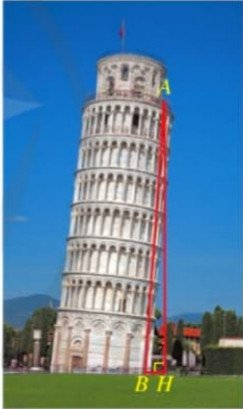
\includegraphics[width=4cm,height=5cm]{images/9C4-3-3.jpg}
	}
	\loigiai{
	Xét tam giác $ABH$ vuông tại $H$, ta có $BH=AH \cdot \tan A=45 \cdot \tan 4 \approx 3{,}15$ (m).\\
	Vậy khoảng cách từ vị trí chạm đất đến chân tháp $3{,}15$ m.
	}
\end{vd}
%%%%% Ước lượng chiều cao
\begin{vd}
	\immini{Các tia nắng mặt trời tạo với mặt đất một góc xấp xỉ bằng $34^\circ$ và bóng của một toà tháp trên mặt đất dài $8{,}6$ m. Tính chiều cao của toà tháp đó (làm tròn đến mét).}
	{
	\begin{tikzpicture}
	\newcommand{\haidang}
	{\tikz{\begin{scope}[scale=.5]
	\fill[violet] (0,0) -- (-5,0) to[out=20,in=180] (-4.3,.15)
	to[out=40,in=180] (-3.05,.65)
	to[out=80,in=200] (-2.8,.85)
	to[out=70,in=160] (-2.3,1.25)
	to[out=50,in=190] (-2,1.45)--(-1.6,1.45)--(-1.35,3.2)--(-1.3,2.15)
	to[out=50,in=210] (0,3.2)
	to[out=28,in=222] (1.25,4.05)--(1.5,1.5)--(1.7,1.5)
	to[out=-40,in=180] (2,1.33)
	to[out=-10,in=110] (2.45,1)
	to[out=-40,in=160] (3,.3)
	to[out=-40,in=150] (3.2,.6)
	to[out=10,in=130] (4.4,.1)
	to[out=0,in=160] (5,0)--cycle
	;
	\fill[violet] (-.85,3.6) rectangle (-.53,4.1);
	\fill[violet] (-1.3,4.2)
	to[out=50,in=208] (0,5.15)
	to[out=25,in=225] (1,5.75)
	to[out=50,in=275] (1.15,6.3)--(1.08,8)
	to[out=-130,in=37] (-1,6.6)
	to[out=-135,in=88] (-1.25,5.5)--cycle
	;
	\fill[violet] (.25,8.45) rectangle (.55,9);
	\fill[violet] (-1.1,8.3)
	to[out=55,in=245] (1.05,9.85)--(1.2,9.85)
	to[out=10,in=263] (1.45,10.1)
	to[out=100,in=-10] (.96,10.35)--(.93,11.1)--(1.05,11.15)
	to[out=155,in=20] (-1.07,11.2)--(-1.07,10.3)
	to[out=-175,in=135] (-1.4,10)
	to[out=-55,in=190] (-1.08,9.85)--cycle
	;
	\draw[violet,line width= 2pt] (.9,11.2)--(.9,11.7)
	(.25,11.2)--(.25,11.9)
	(-.35,11.2)--(-.35,11.9)
	(-1.03,11.2)--(-1.03,11.7)
	to[out=20,in=160] (0.94,11.7)
	(.55,11.8)--(.54,12.7)
	(-.6,11.8)--(-.59,12.7)
	(-.04,11.9)--(-.04,12.7)
	;
	\draw[violet,line width=4pt] (.6,11.2)--(.6,11.3)
	(-.75,11.2)--(-.75,11.3)
	;
	\fill[violet!25] (-.04,12.15) circle (7pt)
	(.6,12.7) arc (0:180:.65 and .7) -- cycle
	(-.04,13.4) circle (5pt)
	;
	\end{scope}}
	}
	\path (0,0) coordinate (A)
	(3.5,0) coordinate (B)
	(3.5,2.75) coordinate (C);
	\node[above,inner sep=0]at (B){\resizebox{!}{2.75cm}{\haidang}};
	\draw (A)--(B)--(C)--cycle;
	\path (A)--(B) node[below,midway]{$8{,}6$ m};
	\path (C)--(B) node[right=0.5cm,midway]{$h$};
	\pic[draw,angle radius=12pt, angle eccentricity=2.25,"$34^\circ$"]{angle=B--A--C};
	\end{tikzpicture}
	}
	\loigiai{
	Ta nhận thấy đường cao của tháp đối diện với góc $34^\circ$ (góc tạo bởi tia nắng mặt trời và bóng của tháp trên mặt đất). Do đó, ta có $h=8,6 \cdot \tan 34^\circ \approx 6$ (m).\\
	Vậy chiều cao của tháp là khoảng $6$ m.
	}
\end{vd}
\begin{vd}
	\immini{Bóng trên mặt đất của một cây dài $25$ m. Tính chiều cao của cây (làm tròn đến dm), biết rằng tia nắng mặt trời tạo với mặt đất góc $40^\circ$.}
	{
	\begin{tikzpicture}
	\definecolor{lightcornflowerblue}{rgb}{0.6, 0.81, 0.93}
	\definecolor{cadmiumgreen}{rgb}{0.0, 0.42, 0.24}
	\definecolor{trueblue}{rgb}{0.0, 0.45, 0.81}
	\definecolor{tumbleweed}{rgb}{0.87, 0.67, 0.53}%màu cát
	\definecolor{forestgreen(web)}{rgb}{0.13, 0.55, 0.13}
	\definecolor{darkpastelgreen}{rgb}{0.01, 0.75, 0.24}
	\definecolor{bronze}{rgb}{0.8, 0.5, 0.2}
	\tikzset{cay/.pic={
	\def\T{ %Thân
	(-.33,0)%trái
	..controls +(-50:.25) and +(40:.45) .. (-.57,-1.45)
	..controls +(20:.1) and +(-160:.15) .. (-.1,-1.3)
	..controls +(-120:.1) and +(60:.15) .. (-.2,-1.6)
	..controls +(-30:.1) and +(-140:.15) .. (.15,-1.3)
	..controls +(-20:.1) and +(-160:.15) .. (.57,-1.4)
	..controls +(170:.4) and +(-160:.1) .. (.35,0)
	..controls +(110:.5) and +(80:.5) .. (-.33,0)
	;}
	%\draw \T;
	\fill[bronze] \T;
	\def\C{ 
	(0,.3)
	..controls +(-100:.25) and +(-60:.2) .. (-.3,.1)
	..controls +(-100:.25) and +(-60:.2) .. (-.6,0)
	..controls +(-120:.45) and +(-110:.35) .. (-1,.2)
	..controls +(-150:.5) and +(-140:.35) .. (-1.15,.7)%nút giao
	..controls +(-170:.4) and +(-170:.35) .. (-1,1.15)
	..controls +(140:.35) and +(110:.4) .. (-.37,1.35)
	..controls +(110:.25) and +(80:.3) .. (-.15,1.35)
	..controls +(80:.3) and +(95:.8) .. (.55,1.1)
	..controls +(80:.2) and +(95:.2) .. (.8,1.1)
	..controls +(20:.1) and +(95:.1) .. (.95,1)
	..controls +(-20:.4) and +(35:.25) .. (1,.47)
	..controls +(-30:.3) and +(-20:.3) .. (.75,0.05)%nút giao
	..controls +(-120:.3) and +(-60:.2) .. (.35,0)
	..controls +(175:.2) and +(-160:.1) .. (.2,0.2)
	..controls +(-160:.1) and +(-70:.1) .. (0,.3)
	;}
	\draw \C;
	\fill[forestgreen(web)] \C;
	\def\C1{ 
	(-1.15,.7)%nút giao
	..controls +(-170:.4) and +(-170:.35) .. (-1,1.15)
	..controls +(140:.35) and +(110:.4) .. (-.37,1.35)
	..controls +(110:.25) and +(80:.3) .. (-.15,1.35)
	..controls +(80:.3) and +(95:.8) .. (.55,1.1)
	..controls +(80:.2) and +(95:.2) .. (.8,1.1)
	..controls +(20:.1) and +(95:.1) .. (.95,1)
	..controls +(-20:.4) and +(35:.25) .. (1,.47)
	..controls +(-50:.5) and +(-85:.6) .. (.65,.55)% gần nút giao
	..controls +(-160:.4) and +(-120:.4) .. (0,.7)
	..controls +(-150:.2) and +(-80:.4) .. (-.63,.6)
	..controls +(-140:.5) and +(-130:.4) .. (-1.15,.7)
	;}
	%\draw \C1;
	\fill[darkpastelgreen] \C1;
	\def\G{ %Gân
	(-.8,.2)
	..controls +(-35:.1) and +(130:.35) .. 
	(-.32,0)%nút giao
	..controls +(-40:.1) and +(45:.35) .. (-.42,-1.25)
	(-.32,0)%nút giao
	..controls +(120:.1) and +(-45:.35) .. (-.58,.45)
	(-.32,0)%nút giao
	..controls +(80:.1) and +(-170:.35) .. (-.05,.45)
	(-.28,.3)
	..controls +(80:.1) and +(-60:.05) .. (-.35,.55)
	%Gân phải
	(.45,-1.3)
	..controls +(130:.6) and +(-160:.3) .. (.6,0.35)
	(.37,0)
	..controls +(35:.2) and +(-150:.1) .. (.66,0.15)
	(.37,0)
	..controls +(80:.2) and +(-40:.1) .. (.18,0.4)
	(.31,0.25)
	..controls +(80:.1) and +(-150:.1) .. (.38,0.5)
	(.25,-0.15)
	..controls +(-110:.05) and +(110:.05) .. (.2,-0.5)%gân dọc
	(.2,-0.25)
	..controls +(-110:.05) and +(110:.05) .. (.17,-0.45)
	(-.2,-0.15)
	..controls +(-70:.1) and +(110:.05) .. (-.18,-0.5)
	(-.15,-0.15)
	..controls +(-70:.1) and +(110:.05) .. (-.15,-0.7)
	(-.05,-0.8)
	..controls +(-80:.15) and +(-10:.15) .. (-.3,-1.28)
	(-.1,-0.9)
	..controls +(-110:.1) and +(20:.05) .. (-.2,-1.1)
	(.1,-1)
	..controls +(-50:.05) and +(120:.05) .. (.15,-1.2)
	(.1,-1.15)
	..controls +(-50:.05) and +(120:.05) .. (.12,-1.2)
	(.15,-.75)
	..controls +(-120:.1) and +(-140:.1) .. (.22,-.9)
	..controls +(70:.12) and +(120:.05) .. (.18,-.9)
	;}
	\draw \G;
	}}
	\path (0,0) coordinate (A)
	(4,0) coordinate (B)
	(4,3.2cm) coordinate (C);
	\path (B)--(C) pic[pos=0.45,scale=1.1]{cay};
	\draw (A)--(B)--(C)--cycle;
	\path (A)--(B) node[below,midway]{$25$ m};
	\pic[draw,angle radius=12pt, angle eccentricity=2.25,"$40^\circ$"]{angle=B--A--C};
	\end{tikzpicture}
	}
	\normalfont
	\loigiai{
	Đổi $25$ m= $250$ dm.\\
	Chiều cao của cây là $25:\cos 40^\circ\approx 326$ dm.
	}
\end{vd}
\begin{vd}
	\immini{Một chiếc máy bay bay lên với vận tốc $500\mathrm{~km/h}$. Đường bay lên tạo với phương nằm ngang một góc $30^\circ$ (Hình bên). Hỏi sau $1{,}2$ phút, máy bay lên cao được bao nhiêu kilômét theo phương thẳng đứng?}
	{
	\begin{tikzpicture}[line cap=round,line join=round,font=\footnotesize]
	\path (0,0) coordinate (A)
	(4,0) coordinate (H)
	(4,{4*tan(30)}) coordinate (B);
	\draw (A)--(B)--(H)--cycle;
	\path ($(A)+(0.5,0.75)$) node[rotate=-15]{\twemoji[scale=0.6]{airplane}};
	\path (A)--(B)node[sloped,pos=0.4,above,scale=0.75]{$500$ km/h};
	\pic[draw,angle radius=12pt,angle eccentricity=2,"$30^\circ$"]{angle=H--A--B};
	\foreach \t/\g in {A/-90,B/90,H/-45}{
	\draw[fill=white] (\t) circle (1pt) node[shift={(\g:7pt)}]{$ \t $};
	}
	\end{tikzpicture}
	}
	\loigiai{
	Trong hình vẽ, $A B$ là đoạn đường máy bay bay lên trong $1{,}2$ phút, $B H$ chính là độ cao máy bay đạt được sau $1{,}2$ phút đó.\\
	Ta có $1{,}2$ phút $=\dfrac{1}{50}$ giờ nên $A B=500 \cdot \dfrac{1}{50}=10~(\mathrm{km} )$.\\
	Tam giác $A B H$ vuông tại $H$, có $\widehat{A}=30^\circ$. Theo Định lí 1, ta có
	\[B H=A B \cdot \sin A=10 \cdot \sin 30^\circ=10 \cdot \dfrac{1}{2}=5~(\mathrm{km}).\]
	Vậy sau $1{,}2$ phút, máy bay lên cao được $5\mathrm{~km}$.
	}
\end{vd}
\begin{vd}
	\immini{
	Một cần cẩu đang nâng một khối gỗ trên sông. Biết tay cẩu $AB$ có chiều dài $16$ m và nghiêng một góc $42^\circ$ so với phương nằm ngang. Tính chiều dài $BC$ của đoạn dây cáp (kết quả làm tròn đến hàng phần mười).
	}
	{
	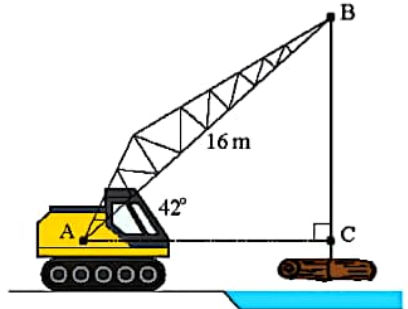
\includegraphics[scale=.6]{images/9S4-2-hinh4}
	}
	\loigiai{
	Xét tam giác $ABC$ vuông tại $C$ có $AB=16$, $\widehat{A}=42^\circ$, ta có:\\
	$BC=AB\cdot \sin A = 16\cdot \sin 42^\circ \approx 10{,}71$ (m).
	}
\end{vd}
\begin{vd}
	Hai con thuyền $P$ và $Q$ cách nhau $300$ m và thẳng hàng với chân $B$ của tháp hải đăng ở trên bờ biển. Từ $P$ và $Q$, người ta nhìn thấy tháp hải đăng dưới các góc $\widehat{BPQ}=14^\circ$ và $\widehat{BQA}=42^\circ$. Đặt $h=AB$ là chiều cao của tháp hải đăng.
	\begin{enumerate}
	\item Tính $BQ$ và $BP$ theo $h$.
	\item Tính chiều cao của tháp hải đăng (kết quả làm tròn đến hàng phần mười).
	\end{enumerate}
	\begin{center}
	\begin{tikzpicture}[line join=round, line cap=round,scale=1,transform shape,>=stealth]
	\definecolor{alizarin}{rgb}{0.82, 0.1, 0.26}
	\definecolor{floralwhite}{rgb}{1.0, 0.98, 0.94}
	\definecolor{brown(traditional)}{rgb}{0.59, 0.29, 0.0}
	\definecolor{bostonuniversityred}{rgb}{0.8, 0.0, 0.0}
	\definecolor{tumbleweed}{rgb}{0.87, 0.67, 0.53}%cát
	\definecolor{deepskyblue}{rgb}{0.0, 0.75, 1.0}
	\definecolor{cerulean}{rgb}{0.0, 0.48, 0.65}
	\definecolor{cadmiumorange}{rgb}{0.93, 0.53, 0.18}
	\tikzset{thuyen_a/.pic={%Buồm
	\def\T{ (.8,1.95)
	..controls +(-140:1.4) and +(85:.5) .. (-1.2,-1.3)
	..controls +(40:.5) and +(100:.65) ..(.8,-1.45)--cycle;}
	\def\M{ (.8,1.95)
	..controls +(-140:1.4) and +(85:.5) .. (-1.2,-1.3)
	..controls +(30:.4) and +(170:.4) ..(.25,-1.05)
	..controls +(85:1.4) and +(-140:.45) .. (.8,1.75);}
	\def\B{ %buồm màu đậm
	(.05,1.15)..controls +(-20:.2) and +(100:.1) .. (.47,0.85)
	..controls +(-130:.01) and +(80:.1) ..(.4,0.37)
	..controls +(130:.01) and +(10:.2) .. (-.25,.7)--cycle
	(-.58,.2)..controls +(-15:.5) and +(100:.1) .. (.33,-.2)--(.28,-.7)
	..controls +(-130:.01) and +(80:.1) ..(-.87,-.35)--cycle;}
	\def\c{ %vòng cung thân thuyền
	(-1.9,-1.2)..controls +(40:.2) and +(150:.1) ..(2.3,-1.2);}
	\def\t{ %thân thuyền
	(-1.3,-2.2)
	..controls +(140:.45) and +(-60:.4) ..(-1.9,-1.2)
	..controls +(-20:1) and +(-150:.5) .. (2.3,-1.2)
	..controls +(-80:.5) and +(60:.4) ..(2,-2.2)
	..controls +(160:.1) and +(-40:.1) ..(1.75,-2.1)
	..controls +(160:.5) and +(-40:.5) ..(.9,-2.1)
	..controls +(160:.5) and +(-40:.5) ..(-.2,-2.1)
	..controls +(160:.5) and +(-40:.5) ..(-1.35,-2.15);}
	\def\S{ %sóng
	(-1.35,-2.15)..controls +(160:.5) and +(-40:.5) ..(-2.5,-2.15)
	(3.5,-2.2)..controls +(160:.2) and +(-40:.5) ..(2,-2.2)
	%----
	(3,-2.5)..controls +(160:.5) and +(-40:.5) ..(1.4,-2.5)
	..controls +(160:.5) and +(-40:.5) ..(.3,-2.5)
	..controls +(160:.5) and +(-40:.5) ..(-.75,-2.55);}
	\draw \c;\draw \t;\draw \T;\draw \M;\draw \B;
	\draw[color=deepskyblue] \S;\fill[cadmiumorange!80] \M;
	\fill[cadmiumorange] \B;\fill[cerulean] \t;
	%Cờ, cột
	\draw[line width=1] (.8,2.4)--(.8,-1.4) ;
	\draw[fill=red] (.8,2.3)--(1.6,2.2)--(.8,1.9)--cycle;}}
	\tikzset{thuyen_b/.pic={%Buồm
	\def\T{ (.8,1.95)
	..controls +(-140:1.4) and +(85:.5) .. (-1.2,-1.3)
	..controls +(40:.5) and +(100:.65) ..(.8,-1.45)--cycle;}
	\def\M{ (.8,1.95)
	..controls +(-140:1.4) and +(85:.5) .. (-1.2,-1.3)
	..controls +(30:.4) and +(170:.4) ..(.25,-1.05)
	..controls +(85:1.4) and +(-140:.45) .. (.8,1.75);}
	\def\B{ %buồm màu đậm
	(.05,1.15)..controls +(-20:.2) and +(100:.1) .. (.47,0.85)
	..controls +(-130:.01) and +(80:.1) ..(.4,0.37)
	..controls +(130:.01) and +(10:.2) .. (-.25,.7)--cycle
	(-.58,.2)..controls +(-15:.5) and +(100:.1) .. (.33,-.2)--(.28,-.7)
	..controls +(-130:.01) and +(80:.1) ..(-.87,-.35)--cycle;}
	\def\c{ %vòng cung thân thuyền
	(-1.9,-1.2)..controls +(40:.2) and +(150:.1) ..(2.3,-1.2);}
	\def\t{ %thân thuyền
	(-1.3,-2.2)
	..controls +(140:.45) and +(-60:.4) ..(-1.9,-1.2)
	..controls +(-20:1) and +(-150:.5) .. (2.3,-1.2)
	..controls +(-80:.5) and +(60:.4) ..(2,-2.2)
	..controls +(160:.1) and +(-40:.1) ..(1.75,-2.1)
	..controls +(160:.5) and +(-40:.5) ..(.9,-2.1)
	..controls +(160:.5) and +(-40:.5) ..(-.2,-2.1)
	..controls +(160:.5) and +(-40:.5) ..(-1.35,-2.15);}
	\def\S{ %sóng
	(-1.35,-2.15)..controls +(160:.5) and +(-40:.5) ..(-2.5,-2.15)
	(3.5,-2.2)..controls +(160:.2) and +(-40:.5) ..(2,-2.2)
	%----
	(3,-2.5)..controls +(160:.5) and +(-40:.5) ..(1.4,-2.5)
	..controls +(160:.5) and +(-40:.5) ..(.3,-2.5)
	..controls +(160:.5) and +(-40:.5) ..(-.75,-2.55);}
	\draw \c;\draw \t;\draw \T;\draw \M;\draw \B;
	\draw[color=deepskyblue] \S;\fill[cadmiumorange!80] \M;
	\fill[red] \B;\fill[cadmiumorange] \t;
	%Cờ, cột
	\draw[line width=1] (.8,2.4)--(.8,-1.4) ;
	\draw[fill=red] (.8,2.3)--(1.6,2.2)--(.8,1.9)--cycle;}}
	%%%%%%%%%%%%%%%%%%%%%%%%%%%%%%%%%%%%%%%%%%%%%%%%%%%%%%
	\tikzset{hai_dang/.pic={
	\draw[line width=1] (0,2.6)--(0,2.4);
	\draw[fill=alizarin] (0,2.4)--(.55,1.86)--(0,1.86);
	\draw[fill=alizarin!95] (0,2.4)--(-.55,1.86)--(0,1.86);
	\draw[fill=alizarin!90] (.6,1.86) rectangle (-.6,1.8);
	\fill[floralwhite!10] (.25,1) rectangle (.5,1.8);
	\fill[floralwhite!40] (0,1) rectangle (.25,1.8);
	\fill[floralwhite!70] (0,1) rectangle (-.25,1.8);
	\fill[floralwhite] (-.25,1) rectangle (-.5,1.8);
	\draw (-.5,1.8) rectangle (.5,1);
	\draw[fill=brown(traditional)!50] (-.55,1.2) rectangle (.55,1);
	\draw[color=brown(traditional)!80, line width=2] 
	(-.6,1)--(-.6,1.33)(-.5,1)--(-.5,1.33)
	(-.4,1)--(-.4,1.33)(-.3,1)--(-.3,1.33)
	(-.15,1)--(-.15,1.33)(.18,1)--(.18,1.33)
	(.35,1)--(.35,1.33)(.5,1)--(.5,1.33)
	(.63,1)--(.63,1.33)(0,1)--(0,1.33);
	\draw[color=brown(traditional)!80, line width=4] 
	(.62,1)--(.4,.5)(-.62,1)--(-.4,.5);
	\fill[floralwhite!70] (-.48,1)--(.48,1)--(.7,-2.6)--(-.7,-2.6)--cycle;
	\fill[bostonuniversityred!80] (-.5,.55)--(-.55,0)--(.55,0)--(.5,.55)--cycle (-.57,-.45)--(-.6,-1.05)--(.6,-1.05)--(.57,-.45)--cycle(-.64,-1.55)--(-.67,-2.1)--(.67,-2.1)--(.64,-1.55)--cycle;
	\draw (-.48,1)--(.48,1)--(.7,-2.6)--(-.7,-2.6)--cycle;
	\draw[fill=brown(traditional)!80](-.05,1) rectangle (.05,.65);
	\draw[fill=brown(traditional)!80](-.65,1.3) rectangle (.65,1.35);
	\draw[fill=brown(traditional)!80](-.65,.94) rectangle (.65,1.05);}}
	\tikzset{cua/.pic={
	\draw[fill=gray!80] (-.1,.1)--(.1,.1)
	..controls +(88:.4) and +(92:.4) ..(-.1,.1);}}
	\fill[red](1,0) circle (.5pt);
	\path 	(2,1.5) coordinate (A)
	(2,-1.6) coordinate (B)
	(-2.1,-1.6) coordinate (Q)
	(-8.1,-1.6) coordinate (P);
	\path(2,0)pic[scale=.6]{hai_dang};
	\path(2,0)pic[scale=.6]{cua};
	\path(2,-.6)pic[scale=.6]{cua};
	\path(2,-1.25)pic[scale=.6]{cua};
	\path(-3,-1)pic[scale=.4]{thuyen_a};
	\path (-9,-1) pic[scale=.4]{thuyen_b};
	\foreach \d/\g in {A/90,B/-90,P/-90,Q/-90}\path[draw,fill=white] (\d) circle(1pt) + (\g:9pt) node {$\d$};
	\draw [very thick] (B)--(P)--(A) (A)--(Q);
	\draw [yellow] (A)--(B);
	\draw pic[draw,angle radius=2mm,thick]{right angle=P--B--A};
	\draw pic[draw,angle radius=4mm,thick]{angle=B--Q--A};
	\draw pic["$42^\circ$",angle radius=14mm]{angle=B--Q--A};
	\draw pic[draw,angle radius=4mm,thick]{angle=B--P--A};
	\draw pic["$14^\circ$",angle radius=18mm,font=\scriptsize]{angle=B--P--A};
	\end{tikzpicture}
	\end{center}
	\loigiai{
	\begin{enumerate}
	\item Xét tam giác $BQA$ vuông tại $B$, ta có $\tan Q=\dfrac{AB}{QB}$ nên $BQ=\dfrac{AB}{\tan 42^\circ} = \dfrac{h}{\tan 42^\circ}$.\\
	Xét tam giác $BPA$ vuông tại $B$, ta có $\tan P=\dfrac{AB}{PB}$ nên $PB=\dfrac{AB}{\tan 14^\circ} = \dfrac{h}{\tan 14^\circ}$.
	\item Ta có $BP-BQ=300$. Suy ra 
	$\begin{aligned}[t]
	&\dfrac{h}{\tan 42^\circ} - \dfrac{h}{\tan 14^\circ} =300\\
	&h=\dfrac{300}{\dfrac{1}{\tan 14^\circ} - \dfrac{1}{\tan 42^\circ}} \approx 103{,}4 \text{ (m).}
	\end{aligned}$\\
	Vậy chiều cao của tháp hải đăng là khoảng $103{,}4$ m.
	\end{enumerate}
	}
\end{vd}
\begin{vd}
	\immini{
	Trong hình bên cho $OH=4$ m, $\widehat{AOH}=42^\circ$, $\widehat{HOB}=28^\circ$. Tính chiều cao $AB$ của cây.
	}
	{
	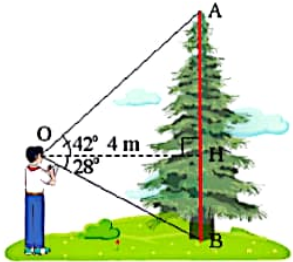
\includegraphics[scale=.75]{images/9S4-2-hinh9}
	}
	\loigiai{
	Xét tam giác $OHA$ vuông tại $H$ ta có $HA=OH \cdot \tan \widehat{HOA} = 4 \cdot \tan 42^\circ \approx 3{,}6$ (m).\\
	Xét tam giác $OHB$ vuông tại $H$ ta có $HB=OH \cdot \tan \widehat{HOB} = 4 \cdot \tan 28^\circ \approx 2{,}1$ (m).\\
	Vậy chiều cao của cây là $AB=HA+HB=3{,}6 + 2{,}1 = 5{,}7$ m.
	}
\end{vd}
\begin{vd}
	\immini{
	Tam giác $ABC$ ở hình bên (có $\widehat{A}= 90^\circ$) mô tả cột cờ $AB$ và bóng nắng của cột cờ trên mặt đất là $AC$. Người ta đo được độ dài $AC = 12$ m và $\widehat{C}= 40^\circ$. Tính chiều cao $AB$ của cột cờ (làm tròn kết quả đến phần trăm của mét).
	}
	{
	\begin{tikzpicture}
	\path (0,0) coordinate (A)--+(3,0) coordinate (C)--++(0,1) coordinate (y)
	($(C)!1!-40:(A)$) coordinate (x)
	(intersection of C--x and A--y) coordinate (B);
	\path pic["\scriptsize$40^\circ$", angle eccentricity=2,draw,angle radius=12pt, double]{angle= B--C--A};
	\draw[line width=2pt, blue] (A)--(B);
	\fill[red] (B) rectangle +(-1,-0.6) node[yellow,midway]{$\bigstar$};
	\draw (A)--(B)--(C)--cyclenode[below,pos=0.5]{$12$ m};
	\foreach \t/\g in {A/180,B/90,C/0}{
	\draw[fill=black] (\t) circle (1pt) node[shift={(\g:7pt)},font=\scriptsize]{$ \t $};
	} 
	\end{tikzpicture}
,	}
	\loigiai{
	Vì tam giác $ABC$ vuông tại $A$ nên $AB =AC\cdot \tan C = 12\cdot \tan 40^\circ \approx 10{,}07$~ (m).
	}
\end{vd}
\begin{vd}
	Trong lần đến tham quan tháp Eiffel (ở Thủ đô Paris, Pháp), bạn Vân muốn ước tính độ cao của tháp. Sau khi quan sát, bạn Vân đã minh hoạ lại kết quả đo đạc ở hình bên. Em hãy giúp bạn Vân tính độ cao $h$ của tháp Eiffel theo đơn vị mét (làm tròn kết quả đến hàng đơn vị).
	\begin{center}
	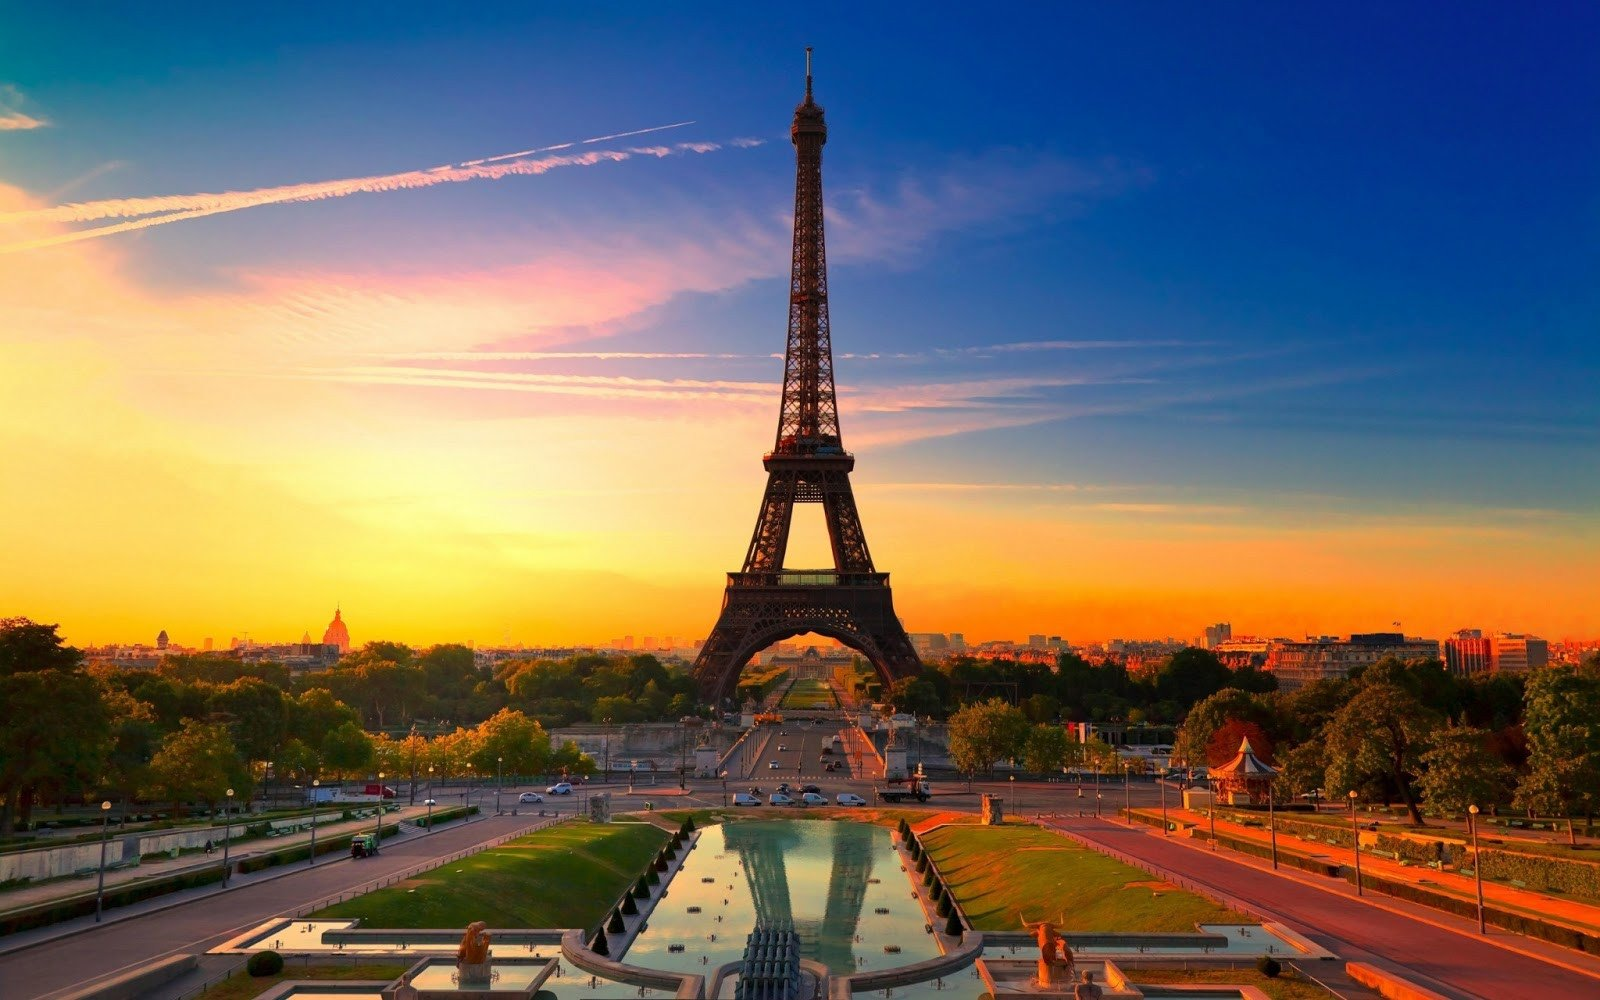
\includegraphics[width=9cm]{images/9C4-3-4.jpg}
	\hspace*{1.5cm}
	\begin{tikzpicture}[>=stealth,line join=round,line cap=round,font=\footnotesize,scale=1]
	\def\c{2.75}	
	\path (0,0) coordinate (A)
	(\c,0) coordinate (C);
	\coordinate (M) at ($(C)!1!-60:(A)$);
	\coordinate (D) at ($(A)!2!(M)$);
	\coordinate (d) at ($(D)!1!-15:(C)$);
	\coordinate (B) at (intersection of A--C and D--d);	
	\draw (D)--(B)--(A)--(D)--(C);
	\draw[dashed] (B)--(C);	
	\foreach \diem/\goc in {D/90,C/-90,B/-90,A/-120}
	{ 
	\fill[black] (\diem) circle (1.5pt) node[shift={(\goc:0.35)}]{$\diem$};
	}
	\draw pic[draw=black,angle radius=5pt] {right angle = A--C--D};
	\draw pic[draw,blue,angle radius=2mm,angle eccentricity=2,"$60^\circ$"] {angle = B--A--D}; 
	\draw pic[draw,double,blue,angle radius=2mm,angle eccentricity=2,"$75^\circ$"] {angle = C--B--D}; 
	\path (D)--(C) node[right,midway]{$h$};
	\path (A)--(B) node[below,midway]{$101$m};
	\end{tikzpicture}
	\end{center}
	\loigiai{
	Xét tam giác $ADC$ vuông tại $C$, ta có: $AC=h\cdot\cot\widehat{DAC}=h\cdot\cot 60^{\circ}$ (m).\\
	Xét tam giác $BDC$ vuông tại $C$, ta có: $B C=h\cdot\cot\widehat{DBC}=h\cdot\cot 75^{\circ}$ (m).\\
	Do $AC-BC=AB=101$ nên
	$h\cdot\cot 60^{\circ}-h\cdot\cot 75^{\circ}=101$ \\
	hay $h\cdot\left(\cot 60^{\circ}-\cot 75^{\circ}\right)=101$ (m).\\
	Suy ra $h=\dfrac{101}{\cot 60^{\circ}-\cot 75^{\circ}}\approx 326$ (m).\\
	Vậy tháp Eiffel có độ cao khoảng $326$ (m).
	}
\end{vd}
\begin{vd}
	\immini{
	Để ước lượng chiều cao của một tháp mà không cần lên đỉnh tháp, người ta sử dụng giác kế, thước cuộn, máy tính cầm tay. Chẳng hạn, ở hình bên, để đo chiều cao $AD$ của tháp, người ta đặt giác kế tại một điểm quan sát cách chân tháp một khoảng $CD=OB=a$, trong đó chiều cao của điểm đặt giác kế là $OC=b$. Quay thanh giác kế sao cho khi ngắm thanh này ta nhìn thấy đỉnh $A$ của tháp, đọc trên giác kế số đo $\alpha$ của góc $AOB$. Tính chiều cao của tháp, biết $\alpha=42^{\circ}$; $b=13{,}81$ m; $a=90$ m (làm tròn kết quả đến hàng phần trăm của mét).
	}{
	\begin{tikzpicture}[scale=0.6, font=\footnotesize, line join = round, line cap = round,>=stealth]
	\def\h{5.5}\def\b{1}\def\a{5}
	\path (0,0) coordinate (D)
	(0,\h) coordinate (A)
	(0,\b) coordinate (B)
	(-\a,\b) coordinate (O)
	(-\a,0) coordinate (C)
	;
	%-------------
	\def\kc{0.6}
	%ống trên
	\fill[ball color=cyan!30] ([xshift=-\kc cm]D)--++(2*\kc,0)--([xshift=0.7*\kc cm,yshift=-3mm]A)coordinate(M1)--++(-1.4*\kc,0)--cycle;
	%ống dưới
	\fill[ball color=cyan] ([xshift=-1.1*\kc cm]D)--++(2.2*\kc,0)--([xshift=0.9*\kc cm,yshift=-2cm]A)--++(-1.8*\kc,0)--cycle;
	%mái trên
	\fill[red] (A)--([xshift=4pt]M1)coordinate(M2)--++(-1.4*\kc cm-8pt,0)--cycle;
	\fill[black] (M2)rectangle+(-1.4*\kc cm-8pt,-2pt);
	%mái giữa
	\fill[red] ([yshift=-1.25cm,xshift=0.7*\kc cm+5pt]A)coordinate(M3) rectangle +(-1.4*\kc cm-10pt,3mm);
	\draw[black,line width=2.5pt] (M3)--++(-1.4*\kc cm-10pt,0);
	%mái dưới
	\fill[red] ([yshift=-2cm,xshift=0.7*\kc cm+7pt]A)coordinate(M4) rectangle +(-1.4*\kc cm-14pt,3.5mm);
	\draw[black,line width=3pt] (M4)--++(-1.4*\kc cm-14pt,0);
	%cửa sổ
	\draw[orange,line width=6pt] (D)++(-0.3*\kc,1.25)--++(0,5mm)
	(D)++(0.3*\kc,2.5)--++(0,5mm);
	%-------------
	\draw[blue, line width=1pt] (A)--(D)--(C)--(O)--cycle;
	\draw[blue,dashed] (B)--(O);
	\draw[dotted] (O)--++(-0.6,0)	(C)--++(-0.6,0) (C)--++(0,-0.6) (D)--++(0,-0.6)
	;
	\draw[red,<->] (C)++(0,-3mm)--++(\a,0) node[below,midway]{$a$};
	\draw[red,<->] (O)++(-3mm,0)--++(0,-\b) node[left,midway]{$b$};
	\foreach \diem/\goc in {A/45,B/0,D/-45,C/-135,O/120}
	{ 
	\fill[black] (\diem) circle (1.5pt) node[shift={(\goc:0.35)}]{$\diem$};
	}
	\draw pic[draw=black,angle radius=5pt] {right angle = O--B--A};
	\draw pic[draw=black,angle radius=5pt] {right angle = C--D--A};
	\draw pic[draw,blue,angle radius=2mm,angle eccentricity=1.8,"$\alpha$"] {angle = B--O--A}; 
	\end{tikzpicture}
	}
	\loigiai{
	Vì tam giác $O A B$ vuông tại $B$ nên
	\begin{eqnarray*}
	AB=OB\cdot\tan\widehat{AOB}=90\cdot\tan 42^{\circ}\approx 81{,}04 \text{ (m).}
	\end{eqnarray*}
	Vậy chiều cao của tháp khoảng
	\begin{eqnarray*}
	81{,}04+13{,}81=94{,}85 \text{ (m).}
	\end{eqnarray*}
	}
\end{vd}
%%%%%%%%%%%%%%%%%%
\subsection{Bài tập vận dụng}
%%%%% Giải tam giác vuông
\begin{bt}
	Giải tam giác $A B C$ vuông tại $A$ có $B C=a$, $A C=b$, $A B=c$, trong các trường hợp
	\begin{listEX}[3]
	\item $a=21$, $b=18$;
	\item $b=10$, $\widehat{C}=30^{\circ}$;
	\item $c=5$, $b=3$.
	\end{listEX}
	\loigiai{
	\begin{center}
	\begin{tikzpicture}[line cap=round,line join=round,font=\footnotesize,scale=0.8]
	\def\r{3}
	\path (0,0) coordinate (O)
	(125:\r) coordinate (A)
	(180:\r) coordinate (B)
	(0:\r) coordinate (C)
	;
	\draw (A)--(B)--(C)--cycle;
	\path (A)--(B) node[midway,left]{$c$};
	\path (A)--(C) node[midway,above]{$b$};
	\path (C)--(B) node[midway,below]{$a$};
	\pic[draw,angle radius=4pt]{right angle=B--A--C};
	\foreach \t/\g in {A/90,B/-135,C/-45}{
	\fill (\t) circle (1pt) node[shift={(\g:7pt)}]{$ \t $};
	}
	\end{tikzpicture}
	\end{center}
	\begin{enumerate}
	\item Tam giác $ABC$ vuông tại $A$ có
	\begin{itemize}
	\item $c=\sqrt{a^2-b^2}=\sqrt{21^2-18^2}=3\sqrt{13}$ (Định lý Pythagoras).
	\item $\cos B=\dfrac{c}{a}=\dfrac{3\sqrt{13}}{21}=\dfrac{\sqrt{13}}{7}\Rightarrow \widehat{B}\approx59^\circ$.
	\item $\widehat{C}=90^\circ-\widehat{B}=90^\circ-59^\circ=31^\circ$.
	\end{itemize}
	\item Tam giác $ABC$ vuông tại $A$ có
	\begin{itemize}
	\item $\widehat{B}=90^\circ-\widehat{C}=90^\circ-30^\circ=60^\circ$
	\item $\cos C=\dfrac{b}{a}\Rightarrow a=\dfrac{b}{\cos C}=\dfrac{10}{\cos 30^\circ}=\dfrac{20\sqrt{3}}{3}$.
	\item $c=\sqrt{a^2-b^2}=\sqrt{\left(\dfrac{20\sqrt{3}}{3}\right)^2-10^2}=\dfrac{10\sqrt{3}}{3}$ (Định lý Pythagoras).
	\end{itemize}
	\item Tam giác $ABC$ vuông tại $A$ có 
	\begin{itemize}
	\item $a=\sqrt{b^2+c^2}=\sqrt{3^2+5^2}=\sqrt{34}$ (Định lý Pythagoras).
	\item $\cos B=\dfrac{c}{a}=\dfrac{5}{\sqrt{34}}\Rightarrow \widehat{B}\approx30{,}96^\circ$.
	\item $\widehat{C}=90^\circ-\widehat{B}=90^\circ-30{,}96^\circ=59{,}04^\circ$.
	\end{itemize}
	\end{enumerate}
	}
\end{bt}
\begin{bt}
	Tìm $x$, $y$ trong mỗi hình bên dưới (làm tròn đến hàng phần mười của centimét).
	\begin{multicols}{3}
	\begin{enumerate}
	\item \begin{center}
	\begin{tikzpicture}[thick, font = \small, scale = 1]
	\path 
	(0,0)coordinate(A)++(0:3)coordinate(B)++(146:1)coordinate(C1)
	($(B)!(A)!(C1)$)coordinate(C)
	;
	\draw (A)--(B)node[midway,below]{$3$ cm}--(C)node[midway,above]{$y$}--(A)node[midway,left]{$x$}
	pic[draw, angle radius = 13pt, "$54^\circ$", angle eccentricity = 1.7]{ angle = B--A--C}
	pic[draw,angle radius = 6pt]{right angle = A--C--B}
	;
	\end{tikzpicture}
	\end{center}
	\item \begin{center}
	\begin{tikzpicture}[thick, font = \small, scale = 1.05]
	\path 
	(0,0)coordinate(A)++(0:3)coordinate(B)++(122:1)coordinate(C1)
	($(B)!(A)!(C1)$)coordinate(C)
	;
	\draw (A)--(B)node[midway,below]{$y$}--(C)node[midway,right]{$1{,}5$ cm}--(A)node[midway,above]{$x$}
	pic[draw, angle radius = 15pt, "$32^\circ$", angle eccentricity = 1.7]{ angle = B--A--C}
	pic[draw,angle radius = 6pt]{right angle = A--C--B}
	;
	\end{tikzpicture}
	\end{center}
	\item \begin{center}
	\begin{tikzpicture}[thick, font = \small, scale = 1.1]
	\path 
	(0,0)coordinate(A)++(0:3.5)coordinate(B)++(160:1)coordinate(C1)
	($(B)!(A)!(C1)$)coordinate(C)
	;
	\draw (A)--(B)node[midway,below]{$x$}--(C)node[midway,above]{$y$}--(A)node[midway,sloped, above]{\small$0{,}8$ cm}
	pic[draw, angle radius = 12pt, "$70^\circ$", angle eccentricity = 1.7]{ angle = B--A--C}
	pic[draw,angle radius = 6pt]{right angle = A--C--B}
	;
	\end{tikzpicture}
	\end{center}
	\end{enumerate}
	\end{multicols}
	\loigiai 
	{
	\begin{enumerate}
	\item Ta có $\sin 54^\circ=\dfrac{y}{3}\Rightarrow y=3\cdot \sin 54^\circ\approx 2{,}4$ (cm).\\
	$\cos 54^\circ=\dfrac{x}{3}\Rightarrow x=3\cdot \cos 54^\circ\approx 1{,}8$ (cm).
	\item Ta có $\sin 32^\circ=\dfrac{1{,}5}{y}\Rightarrow y=\dfrac{1{,}5}{\sin 32^\circ}\approx 2{,}8$ (cm).\\
	$\tan 32^\circ=\dfrac{1{,}5}{x}\Rightarrow x=\dfrac{1{,}5}{\tan 32^\circ}\approx 2{,}4$ (cm).
	\item Ta có $\tan 70^\circ=\dfrac{y}{0{,}8}\Rightarrow y=0{,}8\cdot \tan 70^\circ\approx 2{,}2$ (cm).\\
	$\cos 70^\circ=\dfrac{0{,}8}{x}\Rightarrow x=\dfrac{0{,}8}{\cos 70^\circ}\approx 2{,}3$ (cm).
	\end{enumerate}
	}
\end{bt}
\begin{bt}
	Cho tam giác $ABC$ có đường cao $AH=6$ cm, $\widehat{B}=40^\circ$, $\widehat{C}=35^\circ$. Tính độ dài các đoạn thẳng $AB$, $BH$, $AC$, $BC$ (làm tròn kết quả đến hàng phần mười của centimét).
	\loigiai 
	{
	\immini 
	{
	$\triangle ABH$ vuông tại $H$ có 
	\begin{itemize}
	\item $BH=\dfrac{AH}{\tan 40^\circ}=\dfrac{6}{\tan 40^\circ}\approx 7{,}2$ (cm).
	\item $AB=\dfrac{AH}{\sin 40^\circ}=\dfrac{6}{\sin 40^\circ}\approx 9{,}3$ (cm).
	\end{itemize}
	}
	{
	\begin{tikzpicture}[thick, font = \small, scale = 1]
	\path 
	(0,0)coordinate(B)++(0:5)coordinate(C)++(145:4)coordinate(A)
	($(B)!(A)!(C)$)coordinate(H)
	;
	\draw (A)--(B)--(C)--cycle
	(A)--(H)node[midway,right]{$6$ cm}
	pic[draw, angle radius = 15pt, "$40^\circ$", angle eccentricity = 1.7]{ angle = C--B--A}
	pic[draw,double, angle radius = 15pt, "$35^\circ$", angle eccentricity = 1.7]{ angle = A--C--B}
	pic[draw,angle radius = 6pt]{right angle = A--H--B}
	;
	\foreach \x/\g in {A/90,B/180,C/0,H/-90}
	\fill (\x) circle (1pt)	+(\g:3mm) node{$\x$};
	\end{tikzpicture}
	}
	\noindent
	$\triangle ACH$ vuông tại $H$ có 
	\begin{itemize}
	\item $CH=\dfrac{AH}{\tan 35^\circ}=\dfrac{6}{\tan 35^\circ}\approx 8{,}6$ (cm).
	\item $AC=\dfrac{AH}{\sin 35^\circ}=\dfrac{6}{\sin 35^\circ}\approx 10{,}5$ (cm).
	\end{itemize}
	$BC=BH+HC\approx 7{,}2+8{,}6=15{,}8$ (cm).
	}
\end{bt}
\begin{bt}
	Cho tam giác $ABC$ vuông tại $A$ có $\widehat{B}=30^\circ$. Chứng minh $AC=\dfrac{1}{2}BC$.
	\loigiai 
	{
	\immini 
	{
	Tam giác $ABC$ vuông tại $A$ nên 
	$$\sin B=\dfrac{AC}{BC} \text{ hay } AC=BC\cdot\sin 30^\circ=\dfrac{1}{2}BC.$$
	}
	{
	\begin{tikzpicture}[thick, font = \small, scale = 1]
	\path 
	(0,0)coordinate(A)++(90:2)coordinate(C)++(-30:4)coordinate(B)
	;
	\draw (A)--(B)--(C)--cycle
	pic[draw, angle radius = 15pt, "$30^\circ$", angle eccentricity = 1.7]{ angle = C--B--A}
	pic[draw,angle radius = 6pt]{right angle = B--A--C}
	;
	\foreach \x/\g in {A/180,B/0,C/90}
	\fill (\x) circle (1.5pt)	+(\g:3mm) node{$\x$};
	\end{tikzpicture}
	}
	}
\end{bt}
\begin{bt}
	Cho tam giác $ABC$ vuông cân tại $A$. Chứng minh $AB=AC=\dfrac{\sqrt{2}}{2}BC$.
	\loigiai{
	\immini
	{
	Tam giác $ABC$ vuông cân tại $A$ nên $\widehat{B}=\widehat{C}=45^\circ$.\\
	Ta có $AC=AB=BC\cdot\cos B=BC\cdot\cos 45^\circ=\dfrac{\sqrt{2}}{2}BC$.
	}
	{
	\begin{tikzpicture}[thick, font = \small, scale = 1]
	\path 
	(0:0) coordinate (A)
	+(0:2) coordinate (B)
	($(A)!1!90:(B)$) coordinate (C)
	;
	\draw (A)--(B)--(C)--cycle
	pic[draw,angle radius = 8pt]{right angle = B--A--C}
	;
	\foreach \x/\g in {A/180,B/0,C/90}
	\fill (\x) circle (1.5pt)
	+(\g:3mm) node{$\x$};
	\end{tikzpicture}
	}
	}
\end{bt}
\begin{bt}
	\immini
	{
	Trong hình bên cho $\widehat{O}=\alpha$, $AB=m$ và $\widehat{OAB}=\widehat{OCA}=\widehat{ODC}=90^\circ$. Chứng minh
	\begin{listEX}[3]
	\item $OA=m\cdot\cot\alpha$;
	\item $AC=m\cdot\cos\alpha$;
	\item $CD=m\cdot\cos^2\alpha$.
	\end{listEX}
	}
	{
	\begin{tikzpicture}[thick, font = \small, scale = 1]
	\def\a{3}
	\def\b{2}
	\path 
	(0,0) coordinate (O)++(0:\a) coordinate (A)++(90:\b) coordinate (B)
	($(O)!(A)!(B)$) coordinate (C)
	($(O)!(C)!(A)$) coordinate (D)
	;
	\draw 
	(A)--(O)--(B)--cycle 
	(A)--(C)--(D)
	pic[draw,angle radius = 6pt]{right angle = O--A--B}
	pic[draw,angle radius = 6pt]{right angle = A--C--B}
	pic[draw,angle radius = 6pt]{right angle = A--D--C}
	;
	\path 
	(B)--(A) node [right, midway]{$ m $}
	;
	\draw pic[draw, angle radius = 12pt, "$\alpha$", angle eccentricity = 1.5]{ angle = A--O--B};
	\foreach \x/\g in {A/-90,O/-90,B/90,C/90,D/-90}
	\fill (\x) circle (1pt)	+(\g:3mm) node{$\x$};
	\end{tikzpicture}
	}
	\loigiai{
	\begin{enumerate}
	\item Xét $\triangle OAB$ vuông tại $A$, có $OA=AB\cdot \cot\widehat{BOA}=m\cdot\cot\alpha$.
	\item Ta có $\widehat{BAC}=90^\circ-\widehat{ABC}=90^\circ-\widehat{ABO}=\alpha$.\\
	Xét $\triangle ABC$ vuông tại $C$ có $AC=AB\cdot\cos\widehat{BAC}=m\cdot\cos\alpha$.
	\item Ta có $\widehat{DCA}=90^\circ-\widehat{CAD}=90^\circ-\widehat{CAO}=\alpha$.\\
	Xét $\triangle ACD$ vuông tại $D$ có $CD=AC\cdot\cos\widehat{DCA}=AC\cdot\cos\alpha$.\\
	Mà theo câu $b)$ ta lại có $AC=m\cdot\cos\alpha$ nên $CD=m\cdot\cos^2\alpha$.
	\end{enumerate}
	}
\end{bt}
\begin{bt}
	\immini{
	Tính các cạnh của hình chữ nhật $ABCD$. Biết $AC=16$ cm và $\widehat{BAC}=68^\circ$.
	}
	{
	\begin{tikzpicture}[scale=0.8]
	\def\r{2}
	\path (0,0) coordinate (A)
	(-90:\r) coordinate (B)
	(0:2.5*\r) coordinate (D)
	($(B)+(D)-(A)$) coordinate (C);
	\draw 	(A)--(B)--(C)--(D)--cycle
	(A)--(C) node[midway, above right]{$16$ cm};
	\draw pic[draw,,angle radius=4mm]{angle=B--A--C};
	\draw pic["$68^\circ$",angle radius=12mm]{angle=B--A--C};
	\foreach \x/\g in {A/90,B/-90,C/-90,D/90} \fill[blue] (\x) circle (1pt)($(\g:3mm)+(\x)$) node {$\x$};
	\end{tikzpicture}
	}
	\loigiai{
	Xét tam giác $ABC$ vuông tại $B$, ta có\\
	$AB=AC \cdot \cos \widehat{BAC} = 16 \cdot \cos68^\circ \approx 6$ cm\\
	$BC=AC \cdot \sin \widehat{BAC} = 16 \cdot \sin68^\circ \approx 14{,}8$ cm\\
	Vậy $AB=CD=6$ cm; $AD=BC=14{,}8$ cm.
	}
\end{bt}
%---- Tính góc
\begin{bt}
	Tính các góc của hình thoi có hai đường chéo dài $2\sqrt{3}$ và $2$.
	\loigiai{
	Giả sử hình thoi $ABCD$ có $AC=2\sqrt{3}$, $BD=2$.\\
	Gọi $O$ là giao điểm của $AC$ và $BD$. Khi đó ta có $AC\perp BD$ tại $O$ và $BO=OD=1$; $AO=OC=\sqrt{3}$.\\
	Tam giác $ABO$ vuông tại $O$ có:
	\immini{
	$\tan \widehat{OAB}=\dfrac{BO}{OA}=\dfrac{1}{\sqrt{3}}\Rightarrow \widehat{OAB}=30^\circ$.
	\\ $\widehat{ABO}=90^\circ-\widehat{OAB}=90^\circ-30^\circ=60^\circ$.
	\\
	Suy ra $\widehat{ABC}=\widehat{ACD}=2\cdot \widehat{ABO}=120^\circ$; $\widehat{BAD}=\widehat{BCD}=2\cdot \widehat{BAO}=60^\circ$.}{
		\begin{tikzpicture}[line cap=round,line join=round,font=\scriptsize]
		\path (0,0) coordinate (A)
		({sqrt(3)},1) coordinate (B)
		({2*sqrt(3)},0) coordinate (C)
		({sqrt(3)},-1) coordinate (D)
		(intersection of A--C and B--D) coordinate (O)
		;
		\draw (A)--(B)--(C)--(D)--cycle (A)--(C) (B)--(D);
		\foreach\x/\y in {A/180,B/90,C/0,D/-90,O/45}{\fill (\x) circle (1pt) node[shift={(\y:0.35)}]{$\x$};}
	\end{tikzpicture}
	}
	}
\end{bt}
\begin{bt}
	Cho hình thang $A B C D$ $(A D \parallel B C)$ có $A D=16$ cm, $B C=4$ cm và $\widehat{A}=\widehat{B}=\widehat{A C D}=90^{\circ}$.
	\begin{enumerate}
	\item Kẻ đường cao $C E$ của tam giác $A C D$. Chứng minh $\widehat{ADC}=\widehat{ACE}$. Tính sin của các góc $\widehat{ADC}$, $\widehat{ACE}$ và suy ra $AC^2=AE\cdot AD$. Từ đó tính $AC$.
	\item Tính góc $D$ của hình thang.
	\end{enumerate}
	\loigiai{
	\begin{center}
	\begin{tikzpicture}[scale=0.85]
	\path (0,0) coordinate (A)++(1,0) coordinate (A')
	(0,-3) coordinate (B)
	(2,-3) coordinate (C)
	($(C)!1!-90:(A)$) coordinate (C')
	(intersection of A--A' and C--C') coordinate (D)
	($(A)!(C)!(D)$) coordinate (E)
	;
	\draw (A)--(B)--(C)--(D)--cycle (A)--(C)--(E);
	\pic[draw,angle radius=4pt]{right angle=A--C--D};
	\pic[draw,angle radius=4pt]{right angle=A--B--C};
	\pic[draw,angle radius=4pt]{right angle=B--A--D};
	\pic[draw,angle radius=4pt]{right angle=C--E--D};
	\foreach\x/\y in {A/135,B/-135,C/-45,D/45,E/90}{\fill (\x) circle (1pt) node[shift={(\y:0.35)}]{$\x$};}
	\end{tikzpicture}
	\end{center}
	\begin{enumerate}
	\item Ta có
	\begin{itemize}
	\item $\widehat{ADC}+\widehat{CAD}=90^\circ$ (tam giác $ACD$ vuông tại $C$).
	\item $\widehat{ACE}+\widehat{CAD}=90^\circ$ (tam giác $ACE$ vuông tại $E$).
	\end{itemize}
	Suy ra $\widehat{ADC}=\widehat{ACE}$.\\
	Tam giác $ACD$ vuông tại $C$ có $\sin \widehat{ADC}=\dfrac{AC}{AD}$.\\
	Tam giác $ACE$ vuông tại $E$ có $\sin \widehat{ACE}=\dfrac{AE}{AC}$.\\
	Suy ra $\dfrac{AC}{AE}=\dfrac{AD}{AC}\Rightarrow AC^2=AE\cdot AD$.\\
	Vì tứ giác $AECB$ có $\widehat{B}=\widehat{BAE}=\widehat{AEC}=90^\circ$ nên tứ giác $AECB$ là hình chữ nhật.\\
	$\Rightarrow AE=BC=4$ cm và $AB=CE$.\\
	Ta có $AC^2=AE\cdot AD=4\cdot 16=64\Rightarrow AC=8$ cm.
	\item Ta có $\sin \widehat{ADC}\cdot \sin \widehat{ACE}=\dfrac{AC}{AD}\cdot \dfrac{AE}{AC}=\dfrac{AE}{AD}\Rightarrow \left(\sin \widehat{ADC}\right)^2=\dfrac{4}{16}=\dfrac{1}{4}\Rightarrow \sin \widehat{ADC}=\dfrac{1}{2}$.\\
	Suy ra $\widehat{D}=30^\circ$.
	\end{enumerate}
	}
\end{bt}
\begin{bt}
	Cho tam giác $ABC$ có $BC=20$ cm, $\widehat{ABC}=22^\circ$, $\widehat{ACB}=30^\circ$.
	\begin{enumerate}
	\item Tính khoảng cách từ điểm $B$ đến đường thẳng $AC$.
	\item Tính các cạnh và các góc còn lại của tam giác $ABC$.
	\item Tính khoảng cách từ điểm $A$ đến đường thẳng $BC$.
	\end{enumerate}
	\loigiai{
	\begin{center}
	\begin{tikzpicture}[scale=0.85]
	\def\r{6}
	\path 	(0,0) coordinate (B)
	(0:\r) coordinate (C)
	(B)++(22:.2*\r) coordinate (b)
	(C)++(150:.2*\r) coordinate (c)
	(intersection of B--b and C--c) coordinate (A)
	($(A)!(B)!(C)$) coordinate (H)
	($(B)!(A)!(C)$) coordinate (K);
	\draw 	(A)--(B)--(C)--cycle
	(B)--(H)--(A) (A)--(K);
	\foreach \x/\g in {A/90,B/-90,C/-90,H/90,K/-90} \fill[blue] (\x) circle (1pt)($(\g:3mm)+(\x)$) node {$\x$};
	\foreach\X/\Y/\Z in{B/H/C, A/K/C}\pic[draw,color=blue,angle radius=2mm]{right angle=\X--\Y--\Z};% cần angles
	\end{tikzpicture}
	\end{center}
	\begin{enumerate}
	\item Kẻ $BH \perp AC$ tại $H$.\\
	Xét tam giác $BHC$ vuông tại $H$ ta có $BH=BC\cdot \sin C = 20 \cdot \sin 30^\circ =10$ cm.\\
	Vậy khoảng cách từ $B$ đến $AC$ là $BH=10$ cm.
	\item Xét tam giác $ABC$ ta có 
	$\begin{aligned}[t]
	&\widehat{ABC}+\widehat{ABC}+\widehat{BAC}=180^\circ \\
	&\Rightarrow 22^\circ + 30^\circ + \widehat{BAC} =180^\circ \\
	&\Rightarrow \widehat{BAC} = 180^\circ - 30^\circ - 22^\circ =128^\circ.
	\end{aligned}$\\
	Ta có $\widehat{BAC}+\widehat{BAH}=180^\circ$ (hai góc kề bù)\\
	Suy ra $\widehat{BAH}=180^\circ-\widehat{BAC}=180^\circ-128^\circ = 52^\circ$.\\
	Xét tam giác $AHB$ vuông tại $H$ ta có:\\
	$BH=AB\cdot \sin \widehat{BAH} \Rightarrow AB=\dfrac{BH}{\sin \widehat{BAH}} = \dfrac{10}{\sin 52^\circ} \approx 12{,}7$ (cm).\\
	$HA=BH\cdot \cot \widehat{BAH} = 10 \cdot \cot 52^\circ \approx 7{,}8$ (cm).\\
	Xét tam giác $BHC$ vuông tại $H$ ta có:
	$BC^2=BH^2+HC^2$ (định lí Pythagore)\\
	$\Rightarrow 20^2=10^2+HC^2$\\
	$\Rightarrow HC=\sqrt{20^2-10^2}=10\sqrt{3}$ (cm).\\
	Lại có
	$\begin{aligned}[t]
	&HC=HA+AC \\
	&\Rightarrow AC = HC-HA \\
	&\Rightarrow AC=10\sqrt{3}-7{,}8 \approx 9{,}5 \text{ (cm).}
	\end{aligned}$
	\item Kẻ $AK \perp BC$.\\
	Xét tam giác $AKB$ vuông tại $K$ ta có: $BK = AK \cdot \cot 22^\circ$. \\
	Xét tam giác $AKC$ vuông tại $K$ ta có: $KC = AK \cdot \cot 30^\circ$. \\
	Lại có 
	$\begin{aligned}[t]
	&BC=BK+KC \\
	\Rightarrow & 20=AK \cdot \cot 22^\circ + AK \cdot \cot 30^\circ \\
	\Rightarrow & AK=\dfrac{20}{\cot 22^\circ + \cot 30^\circ} \\
	\Rightarrow & AK\approx 4{,}8 \text{ (cm).}
	\end{aligned}$\\
	Vậy khoảng cách từ $A$ đến $BC$ là $AK \approx 4{,}8$ cm.
	\end{enumerate}
	}
\end{bt}
\begin{bt}
	\immini
	{
	Tính độ dài đường gấp khúc $ABCDEGH$, biết các tam giác $OAB$, $OBC$, $OCD$, $ODE$, $OEG$, $OGH$ là các tam giác vuông tại các đỉnh lần lượt là $B$, $C$, $D$, $E$, $G$, $H$; các góc $O_1$, $O_2$, $O_3$, $O_4$, $O_5$, $O_6$ đều bằng $30^\circ$ và $OA=2$ cm.
	}
	{
	\begin{tikzpicture}[line join=round, line cap=round,scale=1,font=\footnotesize]
	\pgfmathsetmacro \q{0.5*sqrt(3)}
	\path 
	(0,0)coordinate(O)
	(O)++(180:4)coordinate(A)
	(O)++(150:4*\q)coordinate(B)
	(O)++(120:4*\q^2)coordinate(C)
	(O)++(90:4*\q^3)coordinate(D)
	(O)++(60:4*\q^4)coordinate(E)
	(O)++(30:4*\q^5)coordinate(G)
	(O)++(0:4*\q^6)coordinate(H)
	;
	\draw (A)--(B)--(C)--(D)--(E)--(G)--(H)--cycle
	(B)--(O)--(C) 
	(D)--(O)--(G)
	(O)--(E)
	;
	\path
	node at ($(O)+(165:0.5)$){\tiny $1$}
	node at ($(O)+(135:0.5)$){\tiny $2$}
	node at ($(O)+(105:0.5)$){\tiny $3$}
	node at ($(O)+(75:0.5)$){\tiny $4$}
	node at ($(O)+(45:0.5)$){\tiny $5$}
	node at ($(O)+(15:0.5)$){\tiny $6$}
	;
	\foreach \x/\y/\z in {A/B/O,B/C/O,C/D/O,D/E/O,E/G/O,G/H/O}
	\draw pic[draw, angle radius = 6pt]{right angle = \x--\y--\z};
	\foreach \x/\g in {A/-90,B/90,C/90,O/-90,D/90,E/90,G/90,H/0}
	\fill (\x) circle (1pt)	+(\g:3mm) node{$\x$};
	\end{tikzpicture}
	}
	\loigiai{
	\begin{itemize}
	\item Xét $\triangle OAB$ vuông tại $B$ có $\heva{&AB=OA\cdot\sin 30^\circ=2\cdot\sin 30^\circ=1\\&OB=OA\cdot\cos 30^\circ=2\cdot\cos 30^\circ=\sqrt{3}.}$
	\item Xét $\triangle OBC$ vuông tại $C$ có $\heva{&BC=OB\cdot\sin 30^\circ=\sqrt{3}\cdot\sin 30^\circ=\dfrac{\sqrt{3}}{2}\\&OC=OB\cdot\cos 30^\circ=\sqrt{3}\cdot\cos 30^\circ=\dfrac{3}{2}.}$
	\item Xét $\triangle OCD$ vuông tại $D$ có $\heva{&CD=OC\cdot\sin 30^\circ=\dfrac{3}{2}\cdot\sin 30^\circ=\dfrac{3}{4}\\&OD=OC\cdot\cos 30^\circ=\dfrac{3}{2}\cdot\cos 30^\circ=\dfrac{3\sqrt{3}}{4}.}$
	\item Xét $\triangle ODE$ vuông tại $E$ có $\heva{&DE=OD\cdot\sin 30^\circ=\dfrac{3\sqrt{3}}{4}\cdot\sin 30^\circ=\dfrac{3\sqrt{3}}{8}\\&OE=OD\cdot\cos 30^\circ=\dfrac{3\sqrt{3}}{4}\cdot\cos 30^\circ=\dfrac{9}{8}.}$
	\item Xét $\triangle OEG$ vuông tại $G$ có $\heva{&EG=OE\cdot\sin 30^\circ=\dfrac{9}{8}\cdot\sin 30^\circ=\dfrac{9}{16}\\&OG=OE\cdot\cos 30^\circ=\dfrac{9}{8}\cdot\cos 30^\circ=\dfrac{9\sqrt{3}}{16}.}$
	\item Xét $\triangle OGH$ vuông tại $H$ có $GH=OG\cdot\sin 30^\circ=\dfrac{9\sqrt{3}}{16}\cdot\sin 30^\circ=\dfrac{9\sqrt{3}}{32}$.
	\end{itemize}
	Vậy độ dài đường gấp khúc $ABCDEGH$ là
	$$AB+BC+CD+DE+EG+GH=1+\dfrac{\sqrt{3}}{2}+\dfrac{3}{4}+\dfrac{3\sqrt{3}}{8}+\dfrac{9}{16}+\dfrac{9\sqrt{3}}{32}~(\mathrm{cm}).$$
	}
\end{bt}
%%%%%%%%%%%%%%
%%%%% Ứng dụng tính góc
\begin{bt}
	Tính góc nghiêng $\alpha$ của thùng xe chở rác trong hình sau.
	\begin{center}
	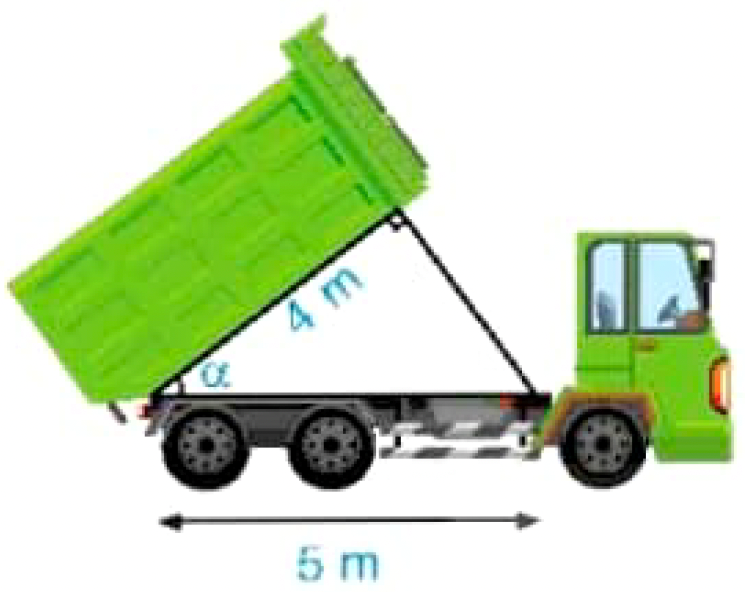
\includegraphics[height=5cm]{images/9T4-12-1}
	\end{center}
	\loigiai{
	Ta có $\cos \alpha =\dfrac{4}{5}\Rightarrow \alpha\approx36{,}87^\circ$.\\
	Vậy góc nghiêng của thùng xe chở rác là khoảng $36{,}87^\circ$.
	}
\end{bt}
\begin{bt}
	Tìm góc nghiêng $\alpha$ và chiều rộng $AB$ của mái nhà kho trong hình sau.
	\begin{center}
	\begin{tikzpicture}[font=\scriptsize,scale=1.2,line cap=round,line join=round]
	\path
	(0,0)coordinate (O)
	(4,0) coordinate (M)
	(0,1) coordinate (N)
	(0,1.3) coordinate (A)
	(4,1) coordinate (B)
	;
	\foreach \a in{A,B,M}{\path ($(\a)+(30:1)$) coordinate (\a');}
	\fill[yellow!20] (O)--(M)--(M')--(B')--(B)--(N)--cycle;
	\fill[gray!25] (A)--(B)--(N)--cycle;
	\filldraw[color=brown!50] (A)--(A')--(B')--(B)--cycle;
	\draw (O)--(M)--(B)--(A)--cycle (A)--(A')--(B')--(B)--cycle (N)--(B)--(B')--(M')--(M);
	\pic[draw,angle radius=6pt]{right angle=A--O--M};
	\pic[draw,angle radius=6pt]{right angle=O--M--B};
	\path (A)--(N)node[midway,left]{$0{,}9$ m};
	\path (O)--(M)node[midway,above]{$15$ m};
	\pic[draw,angle eccentricity=2,"$\tiny \alpha$",angle radius= 1cm ] {angle=A--B--N};
	\foreach \t/\g in {A/160,B/-29}{
	\draw[fill=white] (\t) circle (1pt) node[shift={(\g:7pt)}]{$ \t $};
	}
	\end{tikzpicture}
	\end{center}
	\loigiai{
	Ta có $\tan\alpha =\dfrac{0{,}9}{15}\Rightarrow \alpha \approx3{,}43^\circ$.\\
	Theo Định lý Pythagoras, chiều rộng của mái nhà là $AB=\sqrt{0{,}9^2+15^2}\approx15{,}03$ m.
	}
\end{bt}
%%%%% ứng dụng tính khoảng cách
\begin{bt}
	\immini{
	Trong công việc, người ta cần ước lượng khoảng cách từ vị trí $O$ đến khu đất có dạng hình thang $MNPQ$ nhưng không thể đo được trực tiếp, khoảng cách đó được tính bằng khoảng cách từ $O$ đến đường thẳng $MN$. Người ta chọn vị trí $A$ ở đáy $MN$ và đo được $OA=18 ~\mathrm{m}$, $\widehat{OAN}=44^\circ$. Tính khoảng cách từ vị trí $O$ đến khu đất (làm tròn kết quả đến hàng phần mười của mét).
	}{
	\begin{tikzpicture}[cham/.style={circle,fill=black,inner sep=.7pt},font=\footnotesize,scale=.8]
	\path (0,0) coordinate (M) (5,0) coordinate (N) (4.5,1) coordinate (P) (.5,1) coordinate (Q)
	(1,0) coordinate (A) ++(-44:3.5) coordinate (O) ($(M)!(O)!(N)$) coordinate (B);
	\fill[gray!60] (M)--(N)--(P)--(Q)--cycle;
	\draw (A)node[cham]{}--node[sloped,below]{$18$~m}(O)node[cham]{};	\draw[dashed] (O)--(B)node[cham]{};
	\pic[draw=blue,angle radius=4] {right angle=A--B--O};
	\draw pic["$44^\circ$" scale=.8,draw, angle radius = 10pt,angle eccentricity=1.8]{angle = O--A--B};
	\foreach \i/\j in {A/-120,B/-45,O/-90,M/-120,N/-40,P/40,Q/140} \fill (\i) node[shift={(\j:.22)}]{$\i$};
	\begin{scope}[shift={(2.5,-1.5)},scale=.17]
	\definecolor{maungoai}{RGB}{143,227,255}
	\definecolor{mautrong}{RGB}{176,240,255}
	\definecolor{lua}{RGB}{103,201,25}
	\def\vongngoai{(2.7,3.3) .. controls (4.4,5.3) and (8,5.2) ..
	(9.9,4.2) .. controls (14,3) and (15.1,1.3) ..
	(9.8,.1) .. controls (5.6,-0) and (2.9,0) ..
	(1.4,.4) .. controls (-1.4,1.4) and (0.5,2.3) ..
	(2.7,3.3) -- cycle}
	\tikzset{caylua/.pic={
	\fill[lua]
	(1.1,2.1) -- (1.8,2.1) .. controls (1.7,2.7) and
	(2.3,3.1) .. (2.6,3.5) .. controls (2.4,3.5) and
	(2.2,3.4) .. (2,3.2) -- (2.4,4) .. controls
	(2,3.7) and (1.7,3.5) .. (1.5,3.2) .. controls
	(1.3,3.5) and (1,3.7) .. (0.7,3.9) .. controls
	(0.8,3.6) and (1.1,3.4) .. (1.1,3.2) .. controls
	(0.8,3.4) and (0.6,3.5) .. (0.4,3.6) .. controls
	(0.9,3.1) and (1.2,2.6) .. (1.1,2.1) -- cycle;}}
	\fill[maungoai]\vongngoai;
	\fill[mautrong]
	(3.4,3.3) .. controls (6,5.7) and (8,4.6) ..
	(10.4,3.7) .. controls (13.2,2.7) and (12.5,.6) ..
	(9.8,.5) .. controls (7.2,.5) and (3.9,0) ..
	(2.2,.9) .. controls (0.3,2) and (1.9,2.7) ..
	(3.4,3.3) -- cycle;
	\path (0,.2) pic[rotate=0,scale=.1]{caylua} (9,3) pic[rotate=0,scale=.07]{caylua};
	\end{scope}
	\end{tikzpicture}
	}
	\loigiai{
	Xét $\triangle OAB$ vuông tại $B$, ta có:
	$OB=OA \cdot \sin{A}=18\cdot \sin 44^\circ \approx 12{,}5~\mathrm{m}.$\\
	Vậy khoảng cách từ $O$ đến khu đất là $12{,}5$ m.
	}
\end{bt}

\begin{bt}
	\immini
	{
	Hình bên minh họa một phần con sông có bề rộng\\ $AB=100$ m. Một chiếc thuyền đi thẳng từ vị trí $B$ bên này bờ sông đến vị trí $C$ bên kia bờ sông. Tính quãng đường $BC$ (làm tròn kết quả đến hàng phần mười của mét), biết $\widehat{ABC}=35^\circ$.
	}
	{
	\begin{tikzpicture}[line join=round, line cap=round,scale=1,font=\footnotesize]
	\path 
	(1.5,0)coordinate(A)++(90:3)coordinate(B)
	(A)++(0:1.5)coordinate(C)
	;
	\fill [cyan!50!](0,0)rectangle(5,3)
	;
	\draw
	(A)--(B)node[left,midway]{$100$ m}--(C)--cycle
	pic[draw, angle radius = 20pt, "$35^\circ$", angle eccentricity = 1.5]{ angle = A--B--C}
	pic[draw,angle radius = 6pt]{right angle = C--A--B}
	;
	\foreach \x/\g in {A/-90,B/90,C/-90}
	\fill (\x) circle (1pt)	+(\g:3mm) node{$\x$};
	\end{tikzpicture}
	}
	\loigiai{
	Xét tam giác $ABC$ vuông tại $A$ có $\cos \widehat{ABC}=\dfrac{AB}{BC}$.\\
	Suy ra $BC=\dfrac{AB}{\cos\widehat{ABC}}=\dfrac{100}{\cos 35^\circ}\approx 122{,}1$ (m).
	}
\end{bt}

\begin{bt}
	\immini{Hình  bên mô tả ba vị trí $A$, $B$, $C$ là ba đỉnh của một tam giác vuông và 
	không đo được trực tiếp các khoảng cách từ $C$ đến $A$ và từ $C$ đến $B$. Biết 
	$AB=50$ m, $\widehat{ABC}=40^\circ$. Tính các khoảng cách $CA$ và $CB$ (làm 
	tròn kết quả đến hàng đơn vị của mét).}
	{\begin{tikzpicture}[scale=.4, line join=round, line cap=round, >=stealth]	
	\definecolor{maungoai}{RGB}{143,227,255}
	\definecolor{mautrong}{RGB}{176,240,255}
	\definecolor{lua}{RGB}{103,201,25}
	\def\vongngoai{(2.7,3.3) .. controls (4.4,5.3) and (8,5.2) ..
	(9.9,4.2) .. controls (14,3) and (15.1,1.3) ..
	(9.8,.1) .. controls (5.6,-0) and (2.9,0) ..
	(1.4,.4) .. controls (-1.4,1.4) and (0.5,2.3) ..
	(2.7,3.3) -- cycle}
	\tikzset{caylua/.pic={
	\fill[lua]
	(1.1,2.1) -- (1.8,2.1) .. controls (1.7,2.7) and
	(2.3,3.1) .. (2.6,3.5) .. controls (2.4,3.5) and
	(2.2,3.4) .. (2,3.2) -- (2.4,4) .. controls
	(2,3.7) and (1.7,3.5) .. (1.5,3.2) .. controls
	(1.3,3.5) and (1,3.7) .. (0.7,3.9) .. controls
	(0.8,3.6) and (1.1,3.4) .. (1.1,3.2) .. controls
	(0.8,3.4) and (0.6,3.5) .. (0.4,3.6) .. controls
	(0.9,3.1) and (1.2,2.6) .. (1.1,2.1) -- cycle;}}
	\path (8.5,3) pic[rotate=0,scale=.25]{caylua};
	\path (2,6)coordinate(A)
	++(10,0)coordinate(B)
	(2,5)coordinate(Ay)
	($(B)!1!40:(A)$) coordinate (Bx)
	(intersection of A--Ay and B--Bx) coordinate (C);
	\draw(A)--(B)node[midway,above]{$50$ m}--(C)--cycle;
	\path pic[draw=black,angle radius = 9] {right angle = B--A--C} ;	
	\path pic[draw=black,angle radius = .5cm, angle eccentricity = 1.6,"$40^\circ$"] {angle = A--B--C} ;
	\fill[maungoai]\vongngoai;
	\fill[mautrong]
	(3.4,3.3) .. controls (6,5.7) and (8,4.6) ..
	(10.4,3.7) .. controls (13.2,2.7) and (12.5,.6) ..
	(9.8,.5) .. controls (7.2,.5) and (3.9,0) ..
	(2.2,.9) .. controls (0.3,2) and (1.9,2.7) ..
	(3.4,3.3) -- cycle;
	\path (0,.2) pic[rotate=0,scale=.4]{caylua};
	\begin{scope}
	\clip \vongngoai;
	\draw[thick,dashed](B)--(C)--(A);
	\end{scope}
	\foreach \d/\g in {A/90, B/90, C/-90}	
	\path[draw,fill=white] (\d) circle(1pt) + (\g:15pt) node {$\d$};
	\end{tikzpicture}}
	\loigiai{\allowdisplaybreaks
	\begin{eqnarray*}
	\triangle ABC~\text{vuông tại}~A\\
	\tan\widehat{ABC}&=&\dfrac{AC}{AB}\\
	AC&=&AB\cdot\tan\widehat{ABC}\\
	AC&=&50\cdot\tan 40^\circ\\
	AC&\approx& 42
	\end{eqnarray*}
	\begin{eqnarray*}
	\triangle ABC~\text{vuông tại}~A\\
	\cos\widehat{ABC}&=&\dfrac{AB}{BC}\\
	BC&=&\dfrac{AB}{\cos\widehat{ABC}}\\
	BC&=&\dfrac{50}{\cos 40^\circ}\\
	BC&\approx& 65
	\end{eqnarray*}
	Vậy $CA\approx42$ m và $CB\approx65$ m.
	}
\end{bt}
\begin{bt}
	\immini{
		Một mảnh gỗ có dạng hình chữ nhật $ABCD$ vởi đường chéo $AC=8 ~\mathrm{dm}$. Do bảo quản không tốt nên mảnh gỗ bị hỏng phía hai đỉnh $B$ và $D$. Biết $\widehat{BAC}=64^\circ$. Người ta cần biết độ dài $AB$ và $AD$ để khôi phục lại mảnh gỗ ban đầu. Độ dài $AB$, $AD$ bằng bao nhiêu decimét (làm tròn kết quả đến hàng phần mười)?	
	}{
		\begin{tikzpicture}[font=\footnotesize,scale=1]
			\path (0,0) coordinate (A) (0,2) coordinate (B) (4,2) coordinate (C) (4,0) coordinate (D)
			(0,1.3) coordinate (B1) (.8,2) coordinate (B2) (3.2,0) coordinate (D1) (4,.7) coordinate (D2);
			\fill[orange!20] (A)--(B1) to [out=-30,in=-50] (B2)--(C)--(D2)to [out=150,in=150] (D1)--cycle;
			\draw (A)--node[sloped,above]{$8$~dm}(C)--(D2) (D1)--(A)--(B1) (B2)--(C);	
			\draw[dashed] (B1)--(B)--(B2) (D1)--(D)--(D2);
			\draw pic["$64^\circ$" scale=.8,draw, angle radius = 8pt,angle eccentricity=1.8]{angle = C--A--B};
			\foreach \i/\j in {A/-130,B/130,C/30,D/-30} \fill (\i) circle (1pt) node[shift={(\j:.22)}]{$\i$};
		\end{tikzpicture}	
	}
	\loigiai{
		Xét $\triangle ABC$ vuông tại $B$, ta có:\\
		$AB=AC \cdot \cos A = 8\cdot \cos 64^\circ \approx 3{,}5$ dm.\\
		$BC=AC \cdot \sin A = 8\cdot \sin 64^\circ \approx 7{,}2$ dm.\\
		Vì $ABCD$ là hình chữ nhật nên $AD=BC=7{,}2$ dm.
	}
\end{bt}
\begin{bt}
	\immini
	{
		Từ vị trí $A$ ở phía trên một tòa nhà có chiều cao $AD=68$ m, bác Duy nhìn thấy vị trí $C$ cao nhất của một tháp truyền hình, góc tạo bởi tia $AC$ và tia $AH$ theo phương nằm ngang là $\widehat{CAH}=43^\circ$. Bác Duy cũng nhìn thấy chân tháp tại vị trí $B$ mà góc tạo bởi tia $AB$ và tia $AH$ là $\widehat{BAH}=28^\circ$, điểm $H$ thuộc đoạn thẳng $BC$. Tính khoảng cách $BD$ từ chân tháp đến chân tòa nhà và chiều cao $BC$ của tháp truyền hình (làm tròn kết quả đến hàng phần mười của mét).
	}
	{
		\begin{tikzpicture}[thick, font = \small, scale = 0.7]
			\def\a{2.5}
			\def\b{4}
			\path 
			(0,0) coordinate (D)++(90:\a) coordinate (A)++(0:\b) coordinate (H)
			(D)++(0:\b) coordinate (B)
			($(B)!5/2!(H)$)coordinate(C)
			(A)++(180:0.4)coordinate(A1)
			(D)++(180:0.4)coordinate(D1)
			(C)++(-60:0.5)coordinate(E)++(-90:.5)coordinate(F)++(0:.1)coordinate(G)++(-90:1.5)coordinate(I)++(0:.1)coordinate(J)
			($(D)!(J)!(B)$)coordinate(K)
			(C)++(240:0.5)coordinate(E1)++(-90:.5)coordinate(F1)++(180:.1)coordinate(G1)++(-90:1.5)coordinate(I1)++(180:.1)coordinate(J1)
			($(D)!(J1)!(B)$)coordinate(K1)
			;
			\fill[green!50!] (D)--(A)--(A1)--(D1)--cycle;
			\fill[pattern=horizontal lines] (D)--(A)--(A1)--(D1)--cycle;
			\fill[cyan!40!] (C)--(E)--(F)--(G)--(I)--(J)--(K)--(K1)--(J1)--(I1)--(G1)--(F1)--(E1)--cycle;
			\fill[pattern=grid] (C)--(E)--(F)--(G)--(I)--(J)--(K)--(K1)--(J1)--(I1)--(G1)--(F1)--(E1)--cycle;
			\draw 
			(C)--(E)--(F)--(G)--(I)--(J)--(K)
			(C)--(E1)--(F1)--(G1)--(I1)--(J1)--(K1)
			(A)--(D)node[right,midway]{$68$ m}--(B)
			(A)--(C)--(B)--(A)--(H)
			pic[draw, angle radius = 25pt, "$28^\circ$", angle eccentricity = 1.5]{ angle = B--A--H}
			pic[draw,double, angle radius = 20pt, "$43^\circ$", angle eccentricity = 1.5]{ angle = H--A--C}
			pic[draw,angle radius = 6pt]{right angle = A--D--B}
			pic[draw,angle radius = 6pt]{right angle = A--H--C}
			;
			\foreach \x/\g in {A/90,D/-90,B/-90,H/0,C/90}
			\fill (\x) circle (1pt)
			+(\g:3mm) node{$\x$};
		\end{tikzpicture}
	}
	\loigiai{
		Do $AD\parallel BC$ nên $\widehat{ABD}=\widehat{BAH}=28^\circ$ (so le trong).\\
		Xét $\triangle ABD$ vuông tại $D$ có $BD=AD\cdot\cot\widehat{ABD}=68\cdot\cot 28^\circ\approx 127{,}9$ (m).\\
		Do $ADBH$ là hình chữ nhật nên $BD=AH$ và $AD=BH$.\\
		Xét $\triangle AHC$ vuông tại $H$ có $CH=AH\cdot\tan\widehat{CAH}=127{,}9\cdot \tan 43^\circ\approx 119{,}3$ (m).\\
		Vậy chiều cao của tháp truyền hình là $BC=BH+HC\approx 68+119{,}3=187{,}3$ (m)
	}.
\end{bt}
%%%%% Ứng dụng tính chiều cao
\begin{bt}
	\immini{
		Một người đẩy một vật lên hết một con dốc nghiêng một góc $35^\circ$. Tính độ cao của vật so với mặt đất biết độ dài con dốc là $4$ m.
	}
	{
		\begin{tikzpicture}[=<stealth,scale=0.8]
			\def\r{5}
			\path 	(0,0) coordinate (A)
			(0:1.2*\r) coordinate (B)
			(B)++(90:.7*\r) coordinate (C)
			($(A)!.35!(C)$) coordinate (D)
			($(A)!.6!(C)$) coordinate (E)
			(D)++(120:.2*\r) coordinate (G)
			(E)++(120:.2*\r) coordinate (F)
			(B)++(0:.3) coordinate (b)
			(C)++(0:.3) coordinate (c)
			(A)++(120:.3) coordinate (a)
			(C)++(120:.3) coordinate (d);
			\fill [violet!60] (A)--(C)--(B)--cycle;
			\fill [orange!70!yellow] (D)--(E)--(F)--(G)--cycle;
			\draw (A)--(C) node[midway, below, yshift=-1mm]{$4$ m} --(B)--cycle;
			\draw [<->,thick] (b)--(c) node[midway, right]{?};
			\draw [<->,thick]	(a)--(d);
			\draw pic[draw,,angle radius=6mm]{angle=B--A--C};
			\draw pic["$35^\circ$",angle radius=18mm]{angle=B--A--C};
		\end{tikzpicture}
	}
	\loigiai{
		Độ cao của con dốc so với mặt đất là $4 \cdot \sin 35^\circ \approx 2{,}3$ m.
	}
\end{bt}
\begin{bt}
	Một người đứng tại điểm $A$, cách gương phẳng đặt nằm trên mặt đất tại điểm $B$ là $1{,}2$ m, nhìn thấy hình phản chiếu qua gương $B$ của ngọn cây (cây có góc ở tại điểm $C$ cách $B$ là $4{,}8$ m, $B$ nằm giữa $A$ và $C$). Biết khoảng cách từ mặt đất đến mắt người đó là $1{,}65$ m. Tính chiều cao của cây.
	\begin{center}
	\begin{center}
	\begin{tikzpicture}[line cap=round,line join=round,scale=1,font=\footnotesize]
	\definecolor{lightcornflowerblue}{rgb}{0.6, 0.81, 0.93}
	\definecolor{cadmiumgreen}{rgb}{0.0, 0.42, 0.24}
	\definecolor{trueblue}{rgb}{0.0, 0.45, 0.81}
	\definecolor{tumbleweed}{rgb}{0.87, 0.67, 0.53}%màu cát
	\definecolor{forestgreen(web)}{rgb}{0.13, 0.55, 0.13}
	\definecolor{darkpastelgreen}{rgb}{0.01, 0.75, 0.24}
	\definecolor{bronze}{rgb}{0.8, 0.5, 0.2}
			\tikzset{man/.pic={%
			\fill[brown]
			(1.3,12.6) .. controls (1.2,13.3) and (1.3,13.9) ..
			(1.5,14) .. controls (1.8,14.2) and (2,14.5) ..
			(2.6,14) .. controls (2.6,13.3) and (2.6,12.6) ..
			(2.5,12.5) -- cycle;
			%áo
			\draw[brown,line width=1.4](3.3,11.4) ..controls (3.7,11.7) and (3.8,11.6) .. (4,12.3);
			\fill[cyan!70!white]
			(1.3,12.6) -- (2.5,12.5) -- (2.6,12.2) 
			.. controls	(3.7,12.4) and (3.2,9) .. (3.3,9.6) 
			.. controls	(3.1,9.3) and (3.1,9.4) .. (3.1,9.3) 
			.. controls	(3,9.1) and (2.6,9) .. (2.7,8.4) -- (.8,8.5)
			..	controls (1,8.8) and (1,8.9) .. (1,9.4) 
			.. controls	(0,12) and (.8,12) .. (1.3,12.6)
			;
			%chân
			\fill[brown]
			(.5,6) -- (.3,3.8) -- (.1,.8) -- (.6,.8) --
			(.8,2.6) -- (.9,3.7) -- (1.3,5.7) -- cycle
			(1.7,6) -- (1.6,3.4) -- (1.6,.6) -- (2.3,.9) ..
			controls (2.3,1.6) and (2.2,2.3) .. (2.2,3.3) .. controls
			(2.6,4.4) and (2.5,5.1) .. (2.9,5.8);
			%quần
			\fill[red!50!yellow]
			(.8,8.5) .. controls (.7,8.1) and (.4,7.8) ..
			(.7,6.7) .. controls (.6,6.6) and (.5,6.5) ..
			(.5,5.8) .. controls (.7,5.7) and (1,5.7) ..
			(1.3,5.7) -- (1.4,6.6) -- (1.5,5.8) .. controls
			(2,5.7) and (2.6,5.7) .. (3.1,5.8) .. controls
			(3.1,6.7) and (3,7.5) .. (2.7,8.4) -- cycle;
			%giày
			\fill[cyan!60!yellow]
			(2.3,.9) .. controls (2.7,.6) and (3,.4) ..
			(3.4,.5) .. controls (3.3,.3) and (3.5,.1) ..
			(3.1,0) .. controls (2.6,.1) and (2.2,.1) ..
			(1.7,.1) .. controls (1.5,.3) and (1.6,.4) ..
			(1.6,.6) -- (2.3,.9)
			(0.1,0.8) .. controls (-0.0,0.7) and (-0.0,0.3) ..
			(0.1,0.2) .. controls (0.4,0.2) and (0.8,0.5) ..
			(1.3,0.4) .. controls (1.4,0.5) and (1.3,0.8) ..
			(1.3,0.9) .. controls (1.1,0.7) and (0.9,0.9) ..
			(0.6,0.8) -- (0.1,0.8);}}
	\tikzset{cay/.pic={
	\def\T{ %Thân
	(-.33,0)%trái
	..controls +(-50:.25) and +(40:.45) .. (-.57,-1.45)
	..controls +(20:.1) and +(-160:.15) .. (-.1,-1.3)
	..controls +(-120:.1) and +(60:.15) .. (-.2,-1.6)
	..controls +(-30:.1) and +(-140:.15) .. (.15,-1.3)
	..controls +(-20:.1) and +(-160:.15) .. (.57,-1.4)
	..controls +(170:.4) and +(-160:.1) .. (.35,0)
	..controls +(110:.5) and +(80:.5) .. (-.33,0)
	;}
	%\draw \T;
	\fill[bronze] \T;
	\def\C{ 
	(0,.3)
	..controls +(-100:.25) and +(-60:.2) .. (-.3,.1)
	..controls +(-100:.25) and +(-60:.2) .. (-.6,0)
	..controls +(-120:.45) and +(-110:.35) .. (-1,.2)
	..controls +(-150:.5) and +(-140:.35) .. (-1.15,.7)%nút giao
	..controls +(-170:.4) and +(-170:.35) .. (-1,1.15)
	..controls +(140:.35) and +(110:.4) .. (-.37,1.35)
	..controls +(110:.25) and +(80:.3) .. (-.15,1.35)
	..controls +(80:.3) and +(95:.8) .. (.55,1.1)
	..controls +(80:.2) and +(95:.2) .. (.8,1.1)
	..controls +(20:.1) and +(95:.1) .. (.95,1)
	..controls +(-20:.4) and +(35:.25) .. (1,.47)
	..controls +(-30:.3) and +(-20:.3) .. (.75,0.05)%nút giao
	..controls +(-120:.3) and +(-60:.2) .. (.35,0)
	..controls +(175:.2) and +(-160:.1) .. (.2,0.2)
	..controls +(-160:.1) and +(-70:.1) .. (0,.3)
	;}
	\draw \C;
	\fill[forestgreen(web)] \C;
	\def\C1{ 
	(-1.15,.7)%nút giao
	..controls +(-170:.4) and +(-170:.35) .. (-1,1.15)
	..controls +(140:.35) and +(110:.4) .. (-.37,1.35)
	..controls +(110:.25) and +(80:.3) .. (-.15,1.35)
	..controls +(80:.3) and +(95:.8) .. (.55,1.1)
	..controls +(80:.2) and +(95:.2) .. (.8,1.1)
	..controls +(20:.1) and +(95:.1) .. (.95,1)
	..controls +(-20:.4) and +(35:.25) .. (1,.47)
	..controls +(-50:.5) and +(-85:.6) .. (.65,.55)% gần nút giao
	..controls +(-160:.4) and +(-120:.4) .. (0,.7)
	..controls +(-150:.2) and +(-80:.4) .. (-.63,.6)
	..controls +(-140:.5) and +(-130:.4) .. (-1.15,.7)
	;}
	%\draw \C1;
	\fill[darkpastelgreen] \C1;
	\def\G{ %Gân
	(-.8,.2)
	..controls +(-35:.1) and +(130:.35) .. 
	(-.32,0)%nút giao
	..controls +(-40:.1) and +(45:.35) .. (-.42,-1.25)
	(-.32,0)%nút giao
	..controls +(120:.1) and +(-45:.35) .. (-.58,.45)
	(-.32,0)%nút giao
	..controls +(80:.1) and +(-170:.35) .. (-.05,.45)
	(-.28,.3)
	..controls +(80:.1) and +(-60:.05) .. (-.35,.55)
	%Gân phải
	(.45,-1.3)
	..controls +(130:.6) and +(-160:.3) .. (.6,0.35)
	(.37,0)
	..controls +(35:.2) and +(-150:.1) .. (.66,0.15)
	(.37,0)
	..controls +(80:.2) and +(-40:.1) .. (.18,0.4)
	(.31,0.25)
	..controls +(80:.1) and +(-150:.1) .. (.38,0.5)
	(.25,-0.15)
	..controls +(-110:.05) and +(110:.05) .. (.2,-0.5)%gân dọc
	(.2,-0.25)
	..controls +(-110:.05) and +(110:.05) .. (.17,-0.45)
	(-.2,-0.15)
	..controls +(-70:.1) and +(110:.05) .. (-.18,-0.5)
	(-.15,-0.15)
	..controls +(-70:.1) and +(110:.05) .. (-.15,-0.7)
	(-.05,-0.8)
	..controls +(-80:.15) and +(-10:.15) .. (-.3,-1.28)
	(-.1,-0.9)
	..controls +(-110:.1) and +(20:.05) .. (-.2,-1.1)
	(.1,-1)
	..controls +(-50:.05) and +(120:.05) .. (.15,-1.2)
	(.1,-1.15)
	..controls +(-50:.05) and +(120:.05) .. (.12,-1.2)
	(.15,-.75)
	..controls +(-120:.1) and +(-140:.1) .. (.22,-.9)
	..controls +(70:.12) and +(120:.05) .. (.18,-.9)
	;}
	\draw \G;
	}}
	%\path (B)--(C) pic[pos=0.45,scale=1.1]{cay};
	\path (4,2.7) pic[opacity=0.5,scale=2.1]{cay};
%	\path (-1,0)node[above,inner sep=0pt]{\resizebox{!}{1.2cm}{\color{gray!50}\faMale}};
	\path (-1.3,0) pic[rotate=0,scale=.11]{man};	
	\path (0,0) coordinate (B)
	(-1,0) coordinate (A)
	(-1,1.5) coordinate (D)
	(4,0) coordinate (C)
	(4,6) coordinate (E);
	\draw (A)--(B)--(D) (C)--(B)--(E);
	\pic[draw,angle radius=4pt]{angle=D--B--A};
	\pic[draw,angle radius=4pt]{angle=C--B--E};
	\foreach \x/\y in {A/-90,B/-90,C/-90}{\fill (\x) circle (1pt)node[shift={(\y:0.35)}]{$\x$};}
	\path (A)--(B) node[midway,below]{$1{,}2$};
	\path (C)--(B) node[midway,below]{$4{,}8$};
	\path (D)--(A) node[midway,left=0.25cm]{$1{,}65$};
	\end{tikzpicture}
	\end{center}
	\end{center}
	\loigiai{
	Ta có hình vẽ sau
	\begin{center}
	\begin{tikzpicture}
	\path (0,0) coordinate (B)
	(-1,0) coordinate (A)
	(-1,1.5) coordinate (D)
	(4,0) coordinate (C)
	(4,6) coordinate (E);
	\draw (A)--(B)--(D)--cycle (B)--(C)--(E)--cycle;
	\pic[draw,angle radius=4pt]{right angle=B--A--D};
	\pic[draw,angle radius=4pt]{right angle=B--C--E};
	\pic[draw,angle radius=4pt]{angle=D--B--A};
	\pic[draw,angle radius=4pt]{angle=C--B--E};
	\foreach \x/\y in {A/-90,B/-90,C/-90,D/135,E/45}{\fill (\x) circle (1pt)node[shift={(\y:0.35)}]{$\x$};}
	\end{tikzpicture}
	\end{center}
	Tam giác $ABD$ vuông tại $A$ có $\tan \widehat{ABD}=\dfrac{AD}{AB}$.\\
	Tam giác $BCE$ vuông tại $C$ có $\tan \widehat{CBE}=\dfrac{CE}{BC}$.\\
	Mà $\widehat{ABD}=\widehat{CBE}$.\\
	Nên $\dfrac{AD}{AB}=\dfrac{CE}{BC}\Rightarrow\dfrac{1{,}65}{1{,}2}=\dfrac{CE}{4{,}8}\Rightarrow CE=6{,}6$ m.\\
	Vậy chiều cao của cây là $6{,}6$ m.
	}
\end{bt}

\begin{bt}
	Lúc $6$ giờ sáng, bạn An đi xe đạp từ nhà (điểm $A$) đến trường (điểm $B$). Khi đi từ $A$ đến $B$, An phải đi đoạn lên dốc $AC$ và đoạn xuống dốc $CB$ (Hình dưới). Biết $AB=762$ m, $\widehat{A}=6^\circ$, $\widehat{B}=4^\circ$.
	\begin{center}
			\begin{tikzpicture}
			\def\r{7}
			\path 	(0,0) coordinate (A)
			(0:\r) coordinate (B)
			(18:.4*\r) coordinate (C)
			($(A)!(C)!(B)$) coordinate (H);
			\draw 	(A)--(B)--(C)--cycle
			(C)--(H) node[midway, right]{$h$};
			\draw pic[draw,,angle radius=4mm]{angle=B--A--C};
			\draw pic["$6^\circ$",angle radius=18mm,font=\scriptsize]{angle=B--A--C};
			\draw pic[draw,double,angle radius=12mm]{angle=C--B--A};
			\draw pic["$4^\circ$",angle radius=28mm,font=\scriptsize]{angle=C--B--A};
			\draw pic[draw,angle radius=1.5mm]{right angle=C--H--B};
			\foreach \x/\g in {A/-90,B/-90,C/90,H/-90} \fill[blue] (\x) circle (1pt)($(\g:3mm)+(\x)$) node {$\x$};
		\end{tikzpicture}
	\end{center}
	\begin{enumerate}
	\item Tính chiều cao $h$ của con dốc.
	\item Hỏi bạn An đến trường lúc mấy giờ? Biết rằng tốc độ khi lên dốc là $4$ km/h và tốc độ khi xuống dốc là $19$ km/h.
	\end{enumerate}
	\loigiai{
	\begin{enumerate}
	\item Xét tam giác $AHC$ vuông tại $H$ ta có: $AH = h \cdot \cot 6^\circ$. \\
	Xét tam giác $CHB$ vuông tại $H$ ta có: $HB = h \cdot \cot 4^\circ$. \\
	Lại có 
	$\begin{aligned}[t]
	&AB=AH+HB \\
	\Rightarrow & 762=h \cdot \cot 6^\circ + h \cdot \cot 4^\circ \\
	\Rightarrow & h=\dfrac{762}{\cot 6^\circ + \cot 4^\circ} \\
	\Rightarrow & h\approx 32 \text{ (m).}
	\end{aligned}$\\
	Vậy chiều cao của con dốc là $h \approx 32$ m.
	\item Xét tam giác $AHC$ vuông tại $H$ ta có:\\
	$CH=AC \cdot \sin A \Rightarrow AC=\dfrac{CH}{\sin A}=\dfrac{32}{\sin 6^\circ} \approx 306{,}1$ (m). \\
	Xét tam giác $BHC$ vuông tại $H$ ta có:\\
	$CH=BC \cdot \sin B \Rightarrow BC=\dfrac{CH}{\sin B}=\dfrac{32}{\sin 4^\circ} \approx 458{,}7$ (m).\\
	Đổi $4$ km/h $=\dfrac{10}{9}$ m/s; $19$ km/h $=\dfrac{95}{18}$ m/s.\\
	Thời gian bạn An đi hết quãng đường $AC$ là $\dfrac{306{,}1}{\dfrac{10}{9}} \approx 275{,}5$ (s).\\
	Thời gian bạn An đi hết quãng đường $BC$ là $\dfrac{458{,}7}{\dfrac{95}{18}} \approx 86{,}9$ (s).\\
	Vậy tổng thời gian bạn An đi từ nhà đến trường là $275{,}5 + 86{,}9 =362{,}4$ (s).
	\end{enumerate}
	}
\end{bt}
\begin{bt}
	\immini{Để ước lượng chiều cao của một cây trong sân trường, bạn Hoàng đứng ở sân 
	trường (theo phương thẳng đứng), mắt bạn Hoàng đặt tại vị trí $C$ cách mặt đất 
	một khoảng $CB=DH=1{,}64$ m và cách cây một khoảng $CD=BH=6$ m. Tính chiều cao 
	$AH$ của cây (làm tròn kết quả đến hàng phần trăm của mét), biết góc nhìn 
	$ACD$ bằng $38^\circ$ minh họa ở hình bên.}
	{	\begin{tikzpicture}[scale=1, font=\footnotesize, line join=round, line cap=round, >=stealth]
	\tikzset{treetop/.style = {
	decoration={random steps, segment length=0.4mm},
	decorate
	},trunk/.style = {
	decoration={random steps, segment length=2mm,amplitude=0.2mm},
	decorate}
	}
	\tikzset{man/.pic={%
	\fill[brown]
	(1.3,12.6) .. controls (1.2,13.3) and (1.3,13.9) ..
	(1.5,14) .. controls (1.8,14.2) and (2,14.5) ..
	(2.6,14) .. controls (2.6,13.3) and (2.6,12.6) ..
	(2.5,12.5) -- cycle;
	%áo
	\draw[brown,line width=1.4](3.3,11.4) ..controls (3.7,11.7) and (3.8,11.6) .. (4,12.3);
	\fill[cyan!70!white]
	(1.3,12.6) -- (2.5,12.5) -- (2.6,12.2) 
	.. controls	(3.7,12.4) and (3.2,9) .. (3.3,9.6) 
	.. controls	(3.1,9.3) and (3.1,9.4) .. (3.1,9.3) 
	.. controls	(3,9.1) and (2.6,9) .. (2.7,8.4) -- (.8,8.5)
	..	controls (1,8.8) and (1,8.9) .. (1,9.4) 
	.. controls	(0,12) and (.8,12) .. (1.3,12.6)
	;
	%chân
	\fill[brown]
	(.5,6) -- (.3,3.8) -- (.1,.8) -- (.6,.8) --
	(.8,2.6) -- (.9,3.7) -- (1.3,5.7) -- cycle
	(1.7,6) -- (1.6,3.4) -- (1.6,.6) -- (2.3,.9) ..
	controls (2.3,1.6) and (2.2,2.3) .. (2.2,3.3) .. controls
	(2.6,4.4) and (2.5,5.1) .. (2.9,5.8);
	%quần
	\fill[red!50!yellow]
	(.8,8.5) .. controls (.7,8.1) and (.4,7.8) ..
	(.7,6.7) .. controls (.6,6.6) and (.5,6.5) ..
	(.5,5.8) .. controls (.7,5.7) and (1,5.7) ..
	(1.3,5.7) -- (1.4,6.6) -- (1.5,5.8) .. controls
	(2,5.7) and (2.6,5.7) .. (3.1,5.8) .. controls
	(3.1,6.7) and (3,7.5) .. (2.7,8.4) -- cycle;
	%giày
	\fill[cyan!60!yellow]
	(2.3,.9) .. controls (2.7,.6) and (3,.4) ..
	(3.4,.5) .. controls (3.3,.3) and (3.5,.1) ..
	(3.1,0) .. controls (2.6,.1) and (2.2,.1) ..
	(1.7,.1) .. controls (1.5,.3) and (1.6,.4) ..
	(1.6,.6) -- (2.3,.9)
	(0.1,0.8) .. controls (-0.0,0.7) and (-0.0,0.3) ..
	(0.1,0.2) .. controls (0.4,0.2) and (0.8,0.5) ..
	(1.3,0.4) .. controls (1.4,0.5) and (1.3,0.8) ..
	(1.3,0.9) .. controls (1.1,0.7) and (0.9,0.9) ..
	(0.6,0.8) -- (0.1,0.8);}}
	\path 
	(-5,-2.1) coordinate (C)
	(-5,-3) coordinate (B)
	(0,-3) coordinate (H)
	(0,-2.1) coordinate (D)
	($(C)!1!38:(D)$) coordinate (Cx)
	(intersection of C--Cx and H--D) coordinate (A)	;
	\path ($(B)+(-.2,0)$) pic[rotate=0,scale=.07]{man};	
	\foreach \w/\f in {0.3/30,0.2/50,0.1/70} 
	\fill [brown!\f!black, trunk] (0,0) ++(-\w/2,0) rectangle +(\w,-3);
	\begin{scope}
	\clip(-1,-1.8)--++(2,0)--++(-1,4)--cycle;
	\foreach \n/\f in {1.8/40,1.2/50,1/60,0.7/70,0.6/80,0.4/90}
	\fill [green!\f!black, treetop] ellipse (\n/1.5 and \n);
	\end{scope}	
	\draw (B)--(H)--(D);
	\draw [dashed](B)--(C)node[midway,left]{$1{,}64$ m}--(A)--(D)--(C)node[midway,below]{$6$ m};	
	\pic[draw,"$38^{\circ}$", angle eccentricity=1.4,angle radius=0.8cm]{angle=D--C--A};
	\draw pic[draw, angle radius=2mm]{right angle=B--H--A};
	\draw pic[draw, angle radius=2mm]{right angle=C--D--A};
	\foreach \x/\g in {A/90,B/-90,C/180,H/-90,D/0} 
	\fill[black] (\x)+(\g:.3) node {$\x$};
	\end{tikzpicture}}
	\loigiai{
	\begin{eqnarray*}
	\triangle ACD~\text{vuông tại}~D\\
	\tan\widehat{ACD}&=&\dfrac{AD}{CD}\\
	AD&=&CD\cdot\tan\widehat{ACD}\\
	AD&=&6\cdot\tan 38^\circ\\
	AH&=&AD+DH=6\cdot\tan38^\circ+ 1{,}64\\
	AH&\approx&6{,}33
	\end{eqnarray*}
	Vậy chiều cao của cây $AH\approx6{,}33$ m.
	}
\end{bt}
\begin{bt}
	\immini{
	Trên mặt biển, khi khoảng cách $AB$ từ ca nô đến chân tháp hải đăng là $250 ~\mathrm{m}$, một người đứng trên tháp hải đăng đó nhìn về phía ca nô theo phương $CA$ tạo với phương nằm ngang $Cx$ một góc là $\widehat{ACx}=32^\circ$. Tính chiều cao của tháp hải đăng (làm tròn kết quả đến hàng phần mười của mét), biết $AB \parallel Cx$ và độ cao từ tầm mắt của người đó đến đỉnh tháp hải đăng là $3{,}2 ~\mathrm{m}$.	
	}{
	\begin{tikzpicture}[scale=.2,declare function={h=12;a=h/tan(32);b=(h-2)/tan(32);},font=\scriptsize]
	\fill[teal] (-5,0) 
	to[out=20,in=180] (-4.3,.15)
	to[out=40,in=180] (-3.05,.65)
	to[out=80,in=200] (-2.8,.85)
	to[out=70,in=160] (-2.3,1.25)
	to[out=50,in=190] (-2,1.45)
	--(-1.6,1.45)--(-1.35,3.2)--(-1.3,2.15)
	to[out=50,in=210] (0,3.2)
	to[out=28,in=222] (1.25,4.05)
	--(1.5,1.5)--(1.7,1.5)
	to[out=-40,in=180] (2,1.33)
	to[out=-10,in=110] (2.45,1)
	to[out=-40,in=160] (3,.8)
	to[out=-40,in=150] (3.2,.6)
	to[out=10,in=130] (4.4,.1)
	to[out=0,in=160] (5,0)
	--cycle;
	\fill[teal] (-.85,3.6) rectangle (-.53,4.1);
	\fill[teal] (-1.3,4.2)
	to[out=50,in=208] (0,5.15)
	to[out=25,in=225] (1,5.75)
	to[out=50,in=275] (1.15,6.3)
	--(1.08,8)
	to[out=-130,in=37] (-1,6.6)
	to[out=-135,in=88] (-1.25,5.5)
	--cycle;
	\fill[teal] (.25,8.45) rectangle (.55,9);
	\fill[teal] (-1.1,8.3)
	to[out=55,in=245] (1.05,9.85)--(1.2,9.85)
	to[out=10,in=263] (1.45,10.1)
	to[out=100,in=-10] (.99,10.35)--(.96,11.1)--(1.05,11.15)
	to[out=155,in=20] (-1.07,11.2)--(-1.07,10.3)
	to[out=-175,in=135] (-1.4,10)
	to[out=-55,in=190] (-1.08,9.85)--cycle;
	\draw[teal,line width= 2pt] 
	(.9,11.15)--(.9,11.75)
	(.25,11.35)--(.25,11.9)
	(-.28,11.35)--(-.28,11.9)
	(-1,11.15)--(-1,11.7)
	to[out=20,in=160] (0.94,11.7)
	(.55,11.8)--(.55,12.7)
	(-.58,11.8)--(-.58,12.7)
	(0,11.9)--(0,12.7);
	\draw[teal,line width=4pt] 
	(.6,11.25)--(.6,11.8)
	(-.63,11.25)--(-.63,11.8);
	\fill[teal] (0,12.15) circle (7pt)
	(.65,12.7) arc (0:180:.65) -- cycle
	(0,13.4) circle (5pt);
	\tikzset{Icon-Tau/.pic={
	\fill[ball color=brown!80!cyan!80!white](-4.65,0.08)..controls+(-23:2.5) and+(-165:3.5)..(4.6,0)..controls+(15:0.15) and+(-15:0.5)..(3.9,0.2)..controls+(-172:5) and+(15:2)..(-4.65,0.08);
	%%Thành trong tầu
	\fill[ball color=teal!10!cyan] [red](-4.65,0.08)--+(-25:0.4)..controls+(10:2) and++(-172:5)..(3.8,0)--++(110:0.2)..controls+(-172:5) and+(15:2)..(-4.65,0.08);
	%%Trung tâm tàu
	\fill[ball color=teal!20](-0.25,-0.42)--++(48:1)coordinate(x)--++(-5:0.85)coordinate(y)--++(-112:1.1)coordinate(z)--cycle;
	\fill[ball color=teal!10](x)--(y)--++(0:0.5)coordinate(t)--++(170:1)coordinate(u)--++(180:0.2)--cycle;
	\fill[cyan](t)--++(72:0.7)coordinate(a)--++(175:0.85)coordinate(b)--(u)--cycle;
	\fill[ball color=teal!20!green](a)--++(2:1.2)coordinate(c)--++(165:0.6)--++(-178:1.25)--(b)--cycle;
	\fill[ball color=teal!20](z)--(y)--(t)--(a)--(c)--++(-70:0.4)coordinate(d)--++(2:0.5)coordinate(e)--++(-80:1)--cycle ($(d)!0.5!(c)$)coordinate(m);
	\fill[ball color=teal!20,draw=teal](d)--(e)--(m)--cycle;
	%%Hét trung tâm tàu
	\fill[ball color=teal!90!cyan](-4.65,0.08)..controls+(-23:2.5) and+(-165:3.5)..(4.6,0)..controls+(15:0.05) and++(65:1.2)..(4.2,-1)..controls++(-152:0.75) and+(13:2)..(-1,-2.5)..controls++(-167:1.1) and+(-50:3.5)..(-4.65,0.08);
	\fill[ball color=teal!30!white](2,1.5)--++(80:2)arc(-95:-450:1 and 0.1)--++(-92:2)--cycle;
	\fill[ball color=teal!90!cyan](2,1)coordinate(e)--++(0:0.4)--++(88:0.65)--++(175:0.3)coordinate(f)--cycle;
	\fill[ball color=teal!90!cyan](e)--(f)--++(180:0.2)--++(-115:0.7)--cycle;
	\clip (-4.65,0.08)..controls+(-23:2.5) and+(-165:3.5)..(4.6,0)..controls+(15:0.05) and++(65:1.2)..(4.2,-1)..controls++(-152:0.75) and+(13:2)..(-1,-2.5)..controls++(-167:1.1) and+(-50:3.5)..(-4.65,0.08);
	\fill[red](-4,-0.7)..controls++(-30:2) and++(-160:3)..(4.5,-0.3)--++(-90:0.25)..controls++(-160:3) and++(-25:1.5)..(-3.6,-1.1);
	}}
	\path 
	(0,0) coordinate (B)
	(-b,0) coordinate (A)
	(0,h-2) coordinate (C)
	(A)pic[scale=.1]{Icon-Tau};
	\draw[dashed] (C)--++(180:b)node[above]{$x$};
	\foreach \i/\g in {C/90, A/120, B/-90} \fill (\i)circle(.1) node[shift={(\g:.2)}] {$\i$};
	\draw (A)--(B)node[pos=.5, below]{$250$~m}--(C)--cycle (C) +(-1.5,0) arc (180:212:1.5)node[scale=.7,pos=.75, left=-2pt]{$32^\circ$};
	\end{tikzpicture}	
	}
	\loigiai{
	Xét $\triangle ABC$ vuông tại $B$, có $\widehat{A}=\widehat{ACx}=32^\circ$.\\
	$BC=AB\cdot \tan A=250 \cdot \tan 32^\circ =156{,}2$ m.\\
	Vậy chiều cao của hải đăng là $156{,}2+3{,}2=159{,}4$ m.
	}
\end{bt}